% THIS IS AN EXAMPLE DOCUMENT FOR VLDB 2012
% based on ACM SIGPROC-SP.TEX VERSION 2.7
% Modified by  Gerald Weber <gerald@cs.auckland.ac.nz>
% Removed the requirement to include *bbl file in here. (AhmetSacan, Sep2012)
% Fixed the equation on page 3 to prevent line overflow. (AhmetSacan, Sep2012)

\documentclass{vldb}
\usepackage{graphicx}
\usepackage{balance}  % for  \balance command ON LAST PAGE  (only there!)
\usepackage{listings}% http://ctan.org/pkg/listings
\lstset{
	basicstyle=\ttfamily,
	mathescape
}
\usepackage{booktabs}
\usepackage[caption=false,font=footnotesize]{subfig}
\usepackage{amsmath}
\usepackage{multirow}
\usepackage{enumitem}
\usepackage{color}
\newdef{definition}{Definition}
\newtheorem{theorem}{Theorem}
\newcommand{\tabincell}[2]{\begin{tabular}{@{}#1@{}}#2\end{tabular}}
% Include information below and uncomment for camera ready
\vldbTitle{A Sample Proceedings of the VLDB Endowment Paper in LaTeX Format}
\vldbAuthors{Ben Trovato, G. K. M. Tobin, Lars Th{\sf{\o}}rv{$\ddot{\mbox{a}}$}ld, Lawrence P. Leipuner, Sean Fogarty, Charles Palmer, John Smith, Julius P.~Kumquat, and Ahmet Sacan}
\vldbDOI{https://doi.org/TBD}
\vldbVolume{12}
\vldbNumber{xxx}
\vldbYear{2019}

\begin{document}

% ****************** TITLE ****************************************

\title{A3Log: Automated Asynchronous Evaluation for Recursive Datalog Programs}


% possible, but not really needed or used for PVLDB:
%\subtitle{[Extended Abstract]
%\titlenote{A full version of this paper is available as\textit{Author's Guide to Preparing ACM SIG Proceedings Using \LaTeX$2_\epsilon$\ and BibTeX} at \texttt{www.acm.org/eaddress.htm}}}

% ****************** AUTHORS **************************************

% You need the command \numberofauthors to handle the 'placement
% and alignment' of the authors beneath the title.
%
% For aesthetic reasons, we recommend 'three authors at a time'
% i.e. three 'name/affiliation blocks' be placed beneath the title.
%
% NOTE: You are NOT restricted in how many 'rows' of
% "name/affiliations" may appear. We just ask that you restrict
% the number of 'columns' to three.
%
% Because of the available 'opening page real-estate'
% we ask you to refrain from putting more than six authors
% (two rows with three columns) beneath the article title.
% More than six makes the first-page appear very cluttered indeed.
%
% Use the \alignauthor commands to handle the names
% and affiliations for an 'aesthetic maximum' of six authors.
% Add names, affiliations, addresses for
% the seventh etc. author(s) as the argument for the
% \additionalauthors command.
% These 'additional authors' will be output/set for you
% without further effort on your part as the last section in
% the body of your article BEFORE References or any Appendices.

\numberofauthors{6} %  in this sample file, there are a *total*
% of EIGHT authors. SIX appear on the 'first-page' (for formatting
% reasons) and the remaining two appear in the \additionalauthors section.

\author{
% You can go ahead and credit any number of authors here,
% e.g. one 'row of three' or two rows (consisting of one row of three
% and a second row of one, two or three).
%
% The command \alignauthor (no curly braces needed) should
% precede each author name, affiliation/snail-mail address and
% e-mail address. Additionally, tag each line of
% affiliation/address with \affaddr, and tag the
% e-mail address with \email.
%
% 1st. author
\alignauthor
Ben Trovato\titlenote{Dr.~Trovato insisted his name be first.}\\
       \affaddr{Institute for Clarity in Documentation}\\
       \affaddr{1932 Wallamaloo Lane}\\
       \affaddr{Wallamaloo, New Zealand}\\
       \email{trovato@corporation.com}
% 2nd. author
\alignauthor
G.K.M. Tobin\titlenote{The secretary disavows
any knowledge of this author's actions.}\\
       \affaddr{Institute for Clarity in Documentation}\\
       \affaddr{P.O. Box 1212}\\
       \affaddr{Dublin, Ohio 43017-6221}\\
       \email{webmaster@marysville-ohio.com}
% 3rd. author
\alignauthor Lars Th{\Large{\sf{\o}}}rv{$\ddot{\mbox{a}}$}ld\titlenote{This author is the
one who did all the really hard work.}\\
       \affaddr{The Th{\large{\sf{\o}}}rv{$\ddot{\mbox{a}}$}ld Group}\\
       \affaddr{1 Th{\large{\sf{\o}}}rv{$\ddot{\mbox{a}}$}ld Circle}\\
       \affaddr{Hekla, Iceland}\\
       \email{larst@affiliation.org}
\and  % use '\and' if you need 'another row' of author names
% 4th. author
\alignauthor Lawrence P. Leipuner\\
       \affaddr{Brookhaven Laboratories}\\
       \affaddr{Brookhaven National Lab}\\
       \affaddr{P.O. Box 5000}\\
       \email{lleipuner@researchlabs.org}
% 5th. author
\alignauthor Sean Fogarty\\
       \affaddr{NASA Ames Research Center}\\
       \affaddr{Moffett Field}\\
       \affaddr{California 94035}\\
       \email{fogartys@amesres.org}
% 6th. author
\alignauthor Charles Palmer\\
       \affaddr{Palmer Research Laboratories}\\
       \affaddr{8600 Datapoint Drive}\\
       \affaddr{San Antonio, Texas 78229}\\
       \email{cpalmer@prl.com}
}



\maketitle

\begin{abstract}
Asynchronous recursive processing usually show better performance on convergence speed and resource utilization in many field. However The usage of Asynchronous processing usually be restricted to a small field because of the non-guaranteed correctness and unstable performance. The programming complexity also plagued the user. To address these problem ,we propose a series of \textbf{novel} conditions that how.A3Log. an Asynchronous Graph computing system with a novel asynchronous condition checker embedded, which can  automatically check the whether  user's sequential program can be correctly executed using asynchronous Model.Besides,System provide a simple and convenient datalog interface.Both shared-memory runtime engine and distributed runtime engine. Our results on Amazon EC2 shows that our system shows at least comparable but most of the time better performance against state-of-art graph computing system.
\end{abstract}
\keywords{Asynchronous aggregation, parallel aggregation, recursive program, Datalog}




\section{Introduction}
With the increasing of sensor performance and the rapid expansion of social network data, it is necessary to parallelize or distribute the analysis and computation of large scale data. However, the parallelization of algorithms requires programmers to have a rich knowledge of distributed systems. A large number of big data analysis systems have been proposed which provide high-level language for expressing the computation logic \cite{}. Even so, these systems still require the users to understand the specific programming logic. For example, the typical representative of the BSP computing model, Pregel \cite{} adopts a vertex-centric programming model. It requires programmers to write vertex-centric programs and Explicitly manage the communication.

New interest has recently re-emerged around Datalog for a wide spectrum of knowledge-oriented applications \cite{}%Bigdatalog 25,27,64,47,49}.

Datalog is an excellent candidate language for large-scale data analytics because of its high-level declarative semantics and support for recursion. Datalog's support for recursion makes the expression of data analysis natural \cite{} and its high-level semantics makes it amenable to parallelization and optimization \cite{}.


In recent years, many system research efforts have raised to improve the performance and scalability of Datalog systems. Socialite \cite{socialite} provides a large scale graph evaluation system supporting both sequential and distribute environment. In Socialite, users can define recursive aggregate functions which, as long as they are meet operations, can be evaluated incrementally and efficiently. The \textit{7113340} project provides a full Datalog language implementation and seeks to provide  system supports that optimizes execution over diverse platforms including sequential implementations \cite{Shkapsky:2016:BDA:2882903.2915229}, multi-core machines [59], and clusters \cite{bigdatalog}. It supports relational algebra, aggregation, and recursion, as well as a host of declarative optimizations. MyriaX \cite{Halperin:2014:DMB:2588555.2594530} implements a Datalog System on share-nothing engines based on Myria \cite{}. The computations are incremental, and it support s a variety of iterative models (synchronous, asynchronous, different processing priorities) and failure-handling techniques. It is worth mentioning that MyriaX supports asynchronous processing and shows promising performance for some applications, but it fails to tell in which cases asynchronous processing is suited.

Compared with synchronous recursive processing, asynchronous recursive processing has many advantages, such as fast convergence \cite{}, more efficient resource utilization \cite{}, and priority scheduling \cite{}. However, in practical usage, synchronous systems are more popular than asynchronous systems, which can be attributed to the following three points:

Compared with synchronous recursive processing, asynchronous recursive processing has many advantages, such as fast convergence \cite{}, more efficient resource utilization \cite{}, and priority scheduling \cite{}. However, in practical usage, synchronous systems are more popular than asynchronous systems, which can be attributed to the following three points:

First, \textbf{Non-guaranteed Correctness}. There are several prior works that have employed asynchronous processing engine for improving their system performance. However, these systems only implement asynchronous execution of parallel/distributed algorithms, without any correctness guarantee of the results \cite{}. Asynchronous computation model are blindly used and may result in inconsistent results for convex functions. Maiter \cite{} provides the sufficient conditions for correct asynchronous computations, but these conditions are only suitable in the context of vertex-centric graph computations.

Second, \textbf{More Complexity}. Programmers are used to write sequential programs or synchronous parallel programs. Had the asynchronization conditions been formally given, it is still hard for a non-expert programmer to manually verify these conditions from their programs. In addition, writing asynchronous programs and designing asynchronous systems are even harder, because asynchronous implies disorganized and as a result complicated. Experience from Google \cite{} strongly suggests a synchronous programming model, since asynchronous code is a lot harder to write, tune, and debug.

Third, \textbf{Unstable Performance}. Asynchronous iterative processing avoids the intermediate result coordination phase. The parallel executions of operations are not synchronized and not strictly ordered. This implies that the computations and communications are not under control any more, which may lead to stale computations/communications and potentially reduces the efficiency. The performance gain from asynchronous computation may be not enough to compensate for the performance loss from stale computations/commmunications, leading to unstable performance.


In order to solve these problems, we design and implement a Datalog system supporting automated asynchronous execution, A3Log. Our system is able to automatically check whether a recursive Datalog program can return correct result with asynchronous recursive execution. This is achieved by automated sufficient conditions verification. Maiter \cite{} provides the sufficient conditions for asynchronous graph processing. In this paper, we generalize the sufficient conditions through the analysis of aggregate and non-aggregate operators, which can be easily identified from a user's Datalog program. Aggregate operation is known to be hardly parallelized \cite{distribute aggregate from ms}, while non-aggregate operation can be embarrassingly parallel. Synchronization of parallel computations seems to be the unavoidable coordination step for correct aggregation result though it is known costly. Our new sufficient conditions are provided by analyzing the properties of aggregate operations and non-aggregate operations. A3Log can also automate the condition verification process without user's participation. Further, A3Log provides both shared-memory runtime engine and distributed runtime engine for fast execution.

The contributions of this paper are summarized as follows.
\begin{itemize}
	\item To guarantee the correctness of recursive Datalog program, we clearly define the sufficient conditions that guarantee asynchronous processing to return the same result as synchronous processing through the analysis of aggregate and non-aggregate operators. Even for some recursive programs that do not satisfy these conditions, we propose an approach to conditionally convert them to be qualified for asynchronous aggregation.
	\item To alleviate the burden of programmers, we propose an automated condition verification technique by leveraging satisfiability modulo theories
	(SMT) . User?s sequential program can be automatically checked for asynchronization possibilities and can even be automatically converted to the asynchronous program.
	\item We propose a Datalog implementation, A3Log, to support automated asynchronous aggregation. A3Log is built by modifying distributed Socialite \cite{}. The condition verification techniques are embedded in a Condition Checker component, so that it can asynchronize user's program automatically. A3Log provides both shared-memory runtime engine and distributed runtime engine. The evaluation of a Datalog program are mapped to the update of a distributed hash table structure. By various optimizations, such as concurrency control, priority scheduling, and termination control, users' Datalog programs can be efficiently executed on our system.
	\item We experimentally evaluate A3Log, compared with Socialite [30, 39], GraphLab [33], Myria[49] and Maiter [55].We also perform evaluations with 7 algorithms on 20 more datasets. The experiments are performed on a 32-core instance for many-core experiments and on a cluster with 64 instances for distributed experiments. Our results show that A3Log outperforms other systems in many-core experiments and shows comparable performance with Maiter in distributed experiments. Our results also show that the asynchronous execution of A3Log can achieve 2.25X-222.82X speedup over the synchronous version for various datasets.
\end{itemize}

The rest of the paper are organized as follow: In Sec.2 we describe the details of  automatic asynchronous technology. In Sec.3 we propose a datalog system based on automatic asynchronous the technology .In Section.4  we give the performance evaluation. And then we review the related works in Sec 5 and then conclude the paper in Sec.7

\section{Revisit Aggregate Operation}
\label{sec:aggre}

A \emph{sequential} computation (as opposed to parallel/distributed computation) is composed of a sequence of operations on input. These operations can be classified into two categories, the aggregate operations and the non-aggregate operations. We focus on numerical aggregation in this paper.
 \subsection{Aggregate/Non-Aggregate Operations}
An \emph{\textbf{aggregate operation}} is a function $g()$ that requires more than one variables as input, i.e., $g(X)$ where $X=\{x_1, x_2, \ldots, x_n\}$, and outputs zero or more values. For example, MAX, MIN, SUM, AVG, and COUNT are commonly used aggregate operations. A special but common case is the \emph{\textbf{group-by aggregation}}. A set of input key-value pairs are grouped by key, and the values in each group are aggregated to obtain a new set of key-value pairs. In other words, the group-by aggregation is composed of multiple subset aggregate operations.

On the contrary, a \emph{\textbf{non-aggregate operation}} is a function that takes only one value as input, i.e., $f(x)$, and outputs zero or more values. Since non-aggregate operation only takes one value unit as input, it has the \emph{distributive} property, i.e., $f(x\cup y)=f(x)\cup f(y)$. In essence, the aggregate operation implies a \emph{data fusion}, while a non-aggregate operation implies a \emph{data transformation}.

Note that, the aggregate and non-aggregate operation should be judged according to the number of \emph{variable} inputs instead of constant inputs. For example, the join operation in relational algebra is in general an aggregation since it merges two data sets into one. It takes two inputs $A$ and $B$ and produces one output. However in distributed join implementation, the whole data set $B$ can be small enough to be cached on all distributed workers, which implies that $B$ is a constant input for the distributed join operations. By partitioning and distributing $A$, the join operation is achieved by merging a part of $A$ and the locally cached whole $B$ on each worker. In such a case, the join operation is considered as a non-aggregate operation because each distributed join operation only takes a part of $A$ as a variable input which is different on different processor, where $B$ is the constant for all processors.

\textbf{Parallelization}:Non-aggregate operation only takes one input and does not rely on any other variable, which makes it have the distributive property. By partitioning and distributing the input to many workers, the non-aggregate operations can be embarrassingly parallel \emph{without communication} between workers. Aggregate operation takes multiple inputs which may originate from other workers, so that these aggregate operations or the group-by aggregation can be parallelized but \emph{with communication} between workers. If the inputs for multiple aggregate operations are disjoint, these aggregate operations can be parallelized without communication by carefully partitioning the inputs. However, this is usually impossible since the inputs probably result from the previous computations on other workers and cannot be particularly partitioned.



\subsection{Recursive Aggregation}


\emph{Recursive aggregation} is a sequence of interleaving aggregate and non-aggregate operations where all the aggregate operations are the same and all the non-aggregate operations are the same\footnote{There are also recursive programs without aggregations, which can be embarrassingly parallel.}. It is very common in graph algorithms, data mining and machine learning algorithms. The program with recursive aggregation is referred to as \emph{recursive program}. In this paper, we will focus on optimizing the computations with recursive aggregation.

Let $Y$ denote a set of input variables of aggregate operation $\{y_0,y_1,\dots,y_m\}$and $X$ denote the inputs $\{x_0,x_1,\dots,x_n\}$ of non-aggregate operation.Define $F(X)$ as $\{f(x_0^k) \cup f(x_1^k) \cup \dots \cup f(x_n^k)\}$ that is performing non-aggregation function $f(\dot)$for each item in the set and then combine them. Similarly, We define $G(Y)$as $\{g(Y_0) \cup g(Y_1) \cup \dots \cup g(Y_n)\}$ in which $X_i$ is a subset of inputs X,note that there may be an intersection between any two subsets.Then a recursive program can be represented as follows.
\begin{equation}
\label{eq:recursive2}
\begin{aligned}
Y^{k}=F(X^k),\\
X^{k+1}=G(Y^k)
\end{aligned}
\end{equation}
It  start from $X^0$ in which case the update order is exchanged and an aggregation is first applied. This recursive program terminates when there is no difference between $X^{k+1}$ and $X^k$ or the difference between $X^{k+1}$ and $X^k$ is small enough. Let $(G\circ F)^n$ denote $n$ applications of $(G\circ F)$. The final result of the recursive program is $(G\circ F)^n(X^0)$. Suppose $X$ contains a set of data items, the $F()$ operation can be parallelized with each working on a subset of $X$. The aggregate operation $G()$ can be parallelized if it is a group-by aggregation, but these parallel aggregate operations are synchronized to wait for the complete set of $X^{k+1}$.

\textbf{Example 1: SSSP} The single source shortest path (SSSP) computation is a recursive program that derives the shortest distance from a source node to all other nodes in a graph. The shortest distance is initialized as $+\infty$ for each node except for the source, which is initialized as 0. The $f()$ operation for a node $i$ takes a tuple $\langle i,d_i^k\rangle$ as input where $d_i^k$ is the shortest distance in the $k$th recursion, computes $f(d_i^k)=d_i^k+w_{i,j}=td_j^{k+1}$ for any outgoing neighbors $j$ (where $w_{i,j}$ is the distance from node $i$ to $j$), and outputs the tuples set $\{\langle j,td_j^{k+1}\rangle\}$ and its own $\langle i,d_i^k\rangle$. The aggregate operation $g()$ with respect to each node $j$ takes the input tuples $\{\langle j,td_j^{k+1}\rangle\}$, performs aggregation $g(td_j^{k+1})=min(\{td_j^{k+1}\},d_j^k)=d_j^{k+1}$, and outputs $\langle j,d_j^{k+1}\rangle$. It terminates when all nodes' shortest distances are not changed from previous recursion.

\textbf{Example 2: PageRank} The PageRank computation is another typical recursive program for ranking the nodes in a graph. The ranking score is initialized as $r_i^0=1/|V|$ for each node $i$ where $|V|$ is the total number of nodes. The $f()$ operation for node $i$ takes a tuple $\langle i,r_i^k\rangle$ as input where $r_i^k$ is the ranking score in the $k$th recursion, computes $f(r_i^k)=0.85*r_i^k/d_i=tr_j^{k+1}$ for any outgoing neighbors $j$ (where 0.85 is the constant damping factor and $d_i$ is the out-degree of node $i$), and outputs the tuples set $\{\langle j,tr_j^{k+1}\rangle\}$. The aggregate operation $g()$ with respect to each node $j$ takes the input tuples $\{\langle j,tr_j^{k+1}\rangle\}$, performs aggregation $g(\{tr_j^{k+1}\})=\sum_j{tr_j^{k+1}}+0.15=r_j^{k+1}$ and outputs $\langle j,r_j^{k+1}\rangle$. It terminates when the difference between two continuous recursions' ranking scores is small enough.

\section{Automatic Asynchronous Aggregation}
\label{sec:async}
In this section, we first formally define asynchronous aggregation and introduce accumulated recursive program. We then present how A3 addresses the three concerns of asynchronous aggregation.

\subsection{Asynchronous Aggregation}
\label{sec:async:async}

The recursive program in Equation (\ref{eq:recursive2}) is defined with synchronous aggregation. In parallel or distributed computing, the \emph{synchronous} aggregation means that all the parallel $f()$ operations have to be completed before the next $g()$ operation starts. The $g()$ operation has to be applied on the whole set $X^k$. Correspondingly, we define asynchronous aggregation as follows.

\begin{definition}
	%wqg
	\label{def:asyncaggre}
	(\textbf{Asynchronous Aggregation}) In a recursive program, we assume that the set $X$  is partitioned into $m$ disjoint subsets,and denote $X_i^k$ i.e., $X=\{X_1^k,X_2^k,\ldots,X_m^k\}$, and $\forall i,j, X_i^k\cap X_j^k=\emptyset$. Asynchronous aggregation is to aggregate multiple subsets from different recursions, i.e., $g(X_i^k\cup X_j^{l})$ where $k\neq l$.
\end{definition}

From the definition of recursive aggregation as shown in Equation (\ref{eq:recursive2}), $X^{k+1}$ is resulted from $Y^k$, and $Y^k$ is resulted from $X^k$. $X^{k+1}$ does not exist before applying $g()$ on the complete set of $X^k$. Thus, the asynchronous aggregation $g(X_i^k\cup X_j^{k+1})$ is only possible after $X^{k+1}$ is obtained. In other words, $X^{k+1}$ is a \emph{replacement} of $X^k$ and is closer to the final result. The asynchronous aggregation of $X^{k+1}$ and $X^k$ may result in a wrong result since $X^k$ is a replaced result which is not supposed to be aggregated.

\subsection{Accumulated Recursive Program}
\label{sec:async:accrec}

In order to make asynchronous aggregation feasible, we introduce a particular type of recursive programs.

\begin{definition}
	\label{def:accumasync}
	(\textbf{Accumulated Recursive Program}) Accumulated recursive program is represented as follows.
	\begin{equation}\label{eq:accumasync}
	\begin{aligned}
	\Delta X^{k+1}=(G\circ F)^n(\Delta X^k)
	\end{aligned}
	\end{equation}
	It starts from $\Delta X^0=X^0$ and terminates when The 2-norm of $\Delta X^k$ is 0 or small enough. The final result is the aggregation of all intermediate results, i.e., $X^{k+1}=g(\Delta X^{0} \cup \Delta X^{1} \cup \ldots \cup \Delta X^{k})$. Alternatively, the result can be represented as follows.
	\begin{equation}
	\label{eq:accumasyncres}
	g\Big(\Delta X^0\cup (F\circ G)(\Delta X^0)\cup\ldots\cup (F\circ G)^k(\Delta X^0)\Big).
	\end{equation}
\end{definition}

Intuitively, the accumulated recursive program performs the same computation as normal recursive program, but the final result is the aggregation of all the intermediate results as shown in Equation (\ref{eq:accumasyncres}). The asynchronous aggregation becomes meaningful in accumulated recursive programs, since the final result is the \emph{aggregation} of all recursions' results but not the last recursion's result. Note that, $\Delta X^{k}$ represents the \emph{increment} from previous recursion. This implies that the accumulated recursive program exhibits \textbf{monotonicity}, which has been well studied in the literature \cite{Hellerstein:2010:DIE:1860702.1860704,calm,Lam:2013:SDE:2510649.2511289,Wang:2015:AFR:2824032.2824052}. Briefly speaking, monotonicity means that we only add information, never negate or take away. However, not all recursive programs are monotonic. We have the following theorem to guide the transformation.


\begin{theorem}
	\label{th:monotone}
	(\textbf{Monotonizability}) The accumulated recursive program defined in Equation (\ref{eq:accumasync}) will return the same result as the normal recursive program defined in Equation (\ref{eq:recursive2}), as long as the the following conditions are satisfied.
	\begin{itemize}
		\item \textbf{monotonic}: $g(X)\subseteq f\circ g(X)$;
		\item \textbf{accumulative}: $g(X_1\cup X_2)=g(g(X_1)\cup X_2)$;
		%\item \textbf{commutative}: $g(X_1\cup X_2)=g(X_2\cup X_1)$;
	\end{itemize}
\end{theorem}
Here we provide the formal proof :
 \begin{proof}
  It is known that $Y^k=f(X^k)$and $\Delta X^0=X^0\\$. So we have
 \begin{align}
 &G(\Delta X^0\cup (F\circ G)(\Delta X^0)\cup\ldots\cup (F\circ G)^k(\Delta X^0))\notag \\
 =&g(Y^0\cup f\circ g(Y^0)\cup \ldots \cup (f\circ g)^n(Y^0))    \notag\\
 =&g(g(Y^0)\cup f\circ g(Y^0)\cup \ldots \cup (f\circ g)^n(Y^0))  \tag{1}\\
 =&g(f\circ g(Y^0)\cup (f\circ g)^2(Y^0)\cup \ldots \cup (f\circ g)^n(Y^0)) \tag{2}\\
 =& \ldots \notag \\
 =&g((f\circ g)^n(Y^0))\tag{3}\\
 =&(g \circ f)^n(X^0).\notag
 \end{align}
  Line (1) is true because of the accumulative property. and Line (2) is true because of the monotonic property.
  Repeat applying these two property ,we can reduce all the low order items in turn.
 \end{proof}
 The accumulative property is essential for efficiency execution engine design. If the accumulative condition is satisfied, only the aggregation result $x^k=g(\Delta x^{0},\ldots,\Delta x^{k-1})$ needs to be maintained and is updated by accumulating a new $\Delta x^{k+1}$, i.e., $x^{k+1}=g(x^k,\Delta x^{k})$. Otherwise, the large set $\Delta X^{k}$ needs to be maintained for every recursion $k$. The accumulative property will be used in our system design to save a lot of maintaining cost.

For example, the SSSP computation (Example 1) can be executed as an accumulated recursive program. Its non-aggregate operation $f()$ on node $i$ outputs not only the tuples set $\{\langle j,td_j^{k+1}\rangle\}$ for its outgoing neighbors $j$ but also its previous recursion's aggregation result $\langle i,d_i^k\rangle$. That is, $\{\langle i,td_i^{k+1}\rangle\}$ and $\langle i,d_i^k\rangle$ are contained in $X^{k+1}$, while $\langle i,d_i^k\rangle$ is already contained in $X^{k}$. Hence, $X^{k}\subseteq X^{k+1}$ and the monotonic condition is satisfied. In addition, the aggregate operation $g()$ which is MIN has the accumulative and commutative conditions.


\subsection{Conditions for Asynchronous Aggregation}
\label{sec:async:condition}

As discussed, asynchronous aggregation is possible in accumulated recursive programs. However, not all accumulated recursive programs with asynchronous aggregation will return the same result as that with synchronous aggregation. We demonstrate the sufficient conditions for asynchronous aggregation in the following theorem.

\begin{theorem}
	\label{th:async}
	(\textbf{Asynchronizability}) With asynchronous aggregation, an accumulated recursive program will yield to the same result as with synchronous aggregation, as long as the following order independent condition is satisfied.
	\begin{itemize}
		\item \textbf{order independent}: $g\circ f\circ g(X)=g\circ f(X)$;
	\end{itemize}
\end{theorem}

By asynchronous aggregation, the partial aggregation result is immediately used by the next $f()$ operation. The order independent property implies that no matter the $f()$ operation is first applied or the $g()$ operation is first applied, the effect is the same. As long as the same number of $f()$ operations are applied on all data, the eventual aggregation result will be the same.Here we details the proof:




For the SSSP example, the $f()$ operation expands the BFS searching scope to one-hop-away nodes, and the $g()$ operation picks the minimal distance resulted from the shortest path. The shortest distances are the same no matter making expansion first $g\circ f(X)$ or making aggregation first $f\circ g(X)$, i.e., $min_j(d_j+w)=min_j(d_j)+w$. There are a broad class of computations that satisfy these conditions and can be executed asynchronously (13 programs in Appendix Sec. \ref{sec:app:example}).


\subsection{Conversion Possibilities}
\label{sec:async:convert}

Some non-monotonic computations cannot be written as accumulated recursive program and are not originally qualified for asynchronous aggregation. For example, the PageRank computation cannot be executed as an accumulated recursive program since neither the monotonic condition nor the accumulative condition is satisfied. After applying $f\circ g$ operations, the recursion result $X^{k}$ is replaced by $X^{k+1}$ but not contained in $X^{k+1}$. Further, the aggregate operation $g(\{x_i\})=\sum_i{x_i}+0.15$ does not have the accumulative property due to the additional constant $0.15$.

Fortunately, these computations can be converted to be qualified for asynchronous aggregation. We provide the convertibility conditions as follows.

\begin{theorem}
	\label{th:convert}
	(\textbf{Convertibility}) A recursive program can be converted to an accumulated recursive program for asynchronous aggregation, as long as the recursion performs infinite times and an aggregate operation $g'()$ with the \textbf{accumulative} and \textbf{commutative} properties can be found with the following conditions:
	\begin{itemize}
		\item \textbf{convertible}: $g(X)=g'(X\cup y)$;
		\item \textbf{eliminable}: $lim_{n\rightarrow\infty}(g'\circ f)^n(x)=\textbf{0}$,
\item \textbf{order independent}: $g\circ f\circ g(X)=g\circ f(X)$;
	\end{itemize}
	where the $g'()$ and $f()$ operations are \textbf{order independent} $g'\circ f\circ g'(X)=g'\circ f(X)$, $y$ is a constant value, and \textbf{0} is the identity element of the $g'()$ operation. The $g'()$ operation is the aggregate operation in the new accumulated recursive program.
\end{theorem}

The formal proof can be found in Appendix Sec. \ref{sec:app:proof:convert}. We present the intuition as follows. We aim to find a new aggregate operation $g'()$ that is with an additional constant input value $y$ but always returns the same result as $g()$, i.e., $g(X)=g'(X\cup y)$. The constant input implies the set containment relation between result and input, which makes it satisfy the monotonic condition that is required for accumulated recursive program. In addition, the eliminable property guarantees the accumulated recursive program to converge, such that the result is independent of $X$. Note that, it is not realistic to perform recursion infinite times. In practice, we will stop the recursion as long as $(g'\circ f)^n(x)$ is ``small'' enough.

For example, PageRank is such an iterative algorithm that can be converted to the accumulated recursive form \cite{maiter}. In original PageRank, $g(\{x_j\})=\sum_j{x_j}+0.15$. The $g()$ function can be rewritten as $g(X)=g'(X\cup y)$ where the $g'()$ function can be ``SUM'', $X=\{x_j\}$ is the input values set, and the constant value $y$ can be 0.15. Apparently, $g'()$ (i.e., ``SUM'') has the accumulative and commutative property. In addition, the $f()$ operation in PageRank contains a constant damping factor 0.85, which leads to $(g'\circ f)(x)<x$ and $lim_{n\rightarrow\infty}(g'\circ f)^n(x)=0$. Furthermore, the $f()$ operation and $g'()$ operation in PageRank is order independent, which makes it suitable for asynchronous aggregation. The resulted ranking scores are the same no matter making decay first $g\circ f(X)$ or making summation first $f\circ g(X)$, i.e., $\sum_j(0.85*\frac{r_j}{d})=0.85*\frac{\sum_j(r_j)}{d}$. There exist other convertable algorithms, such as Program 13 Jacobi Method in Appendix Sec. \ref{sec:app:example}.


\subsection{Automatic Asynchronization}
\label{sec:async:autoasync}

Though the conditions for asynchronous aggregation have been identified, it is still hard for a non-expert programmer to verify these conditions manually. It is even harder to find an aggregate function $g'()$ in order to convert a normal recursive program to an accumulated recursive program. To alleviate the burden of programmers, an automatic asynchronization scheme is desired. In this subsection, we discuss how to automatically verify these conditions given the $g()$ and $f()$ operations\footnote{The $g$ and $f$ operations in Datalog programs can be identified as will be shown in next section.}.

The condition verification problem can be thought of as a form of the constraint satisfaction problem, which can be analyzed with the help of \emph{satisfiability modulo theories} (SMT) \cite{53e486195688442995f82bfe28c55731}. The satisfiability of these conditions can then be checked by an SMT solver, such as Z3 \cite{DeMoura:2008:ZES:1792734.1792766}. Next, we show how to reduce these condition verification problems into SMT satisfiability solving problems.

First, the $f()$ and $g()$ functions and the conditions have to be translated into a formula for being verified by an SMT solver. Given a function $F=f(x_1)$ or $F=g(x_1,\ldots,x_n)$, we are interested in a formula for $F$ of the form $\phi_F^{o_1,\ldots,o_m}$, where $o_1,\ldots,o_m$ are output variables \cite{Liu:2014:ADP:2670979.2670980}. Intuitively, the formula $\phi$ is ``correct'' if an assignment to $\{x_1,\ldots,x_n,o_1,\ldots,o_m\}$ makes $\phi$ be true if and only evaluating $F(x_1,\ldots,x_n)$ returns $o_1,\ldots,o_m$. Then the satisfiability of $\phi$ exactly implies that the function will compute the same output. Based on this formula, we present the formulas for different conditions in the following.

For the accumulative and commutative conditions in Theorem \ref{th:monotone} and the order independent condition in Theorem \ref{th:async}, the condition verification problems can be reduced to SMT satisfiability problems via the following theorem.

\begin{theorem}
	\label{th:auto:1}
	(\textbf{Accumulative, Commutative, and Order Independent}) $\forall x_1,x_2,x_3$, the condition 1 or 2 or 3 is true if and only if $\phi_{F_l}^{o1,\ldots,o_m}\wedge \phi_{F_r}^{o_1',\ldots,o_m'}\wedge (\vee_{i=1}^m{o_i\neq o_i'})$ is not satisfiable, where
	\begin{itemize}
		\item condition 1: accumulative, $F_l=g(x_1,x_2,x_3)$ and $F_r=g(g(x_1,x_2),x_3)$;
		\item condition 2: commutative, $F_l=g(x_1,x_2)$ and $F_r=g(x_2,x_1)$;
		\item condition 3: order independent, $F_l=g(f(g(x_1,x_2)))$ and $F_r=g(f(x_1),f(x_2))$.
	\end{itemize}
\end{theorem}

In the theorem, $\wedge$ denotes AND operator and $\vee$ denotes OR operator. Note that, SMT solver cannot answer ``whether a formula $F$ is always true?'' but only answers ``whether a formula $F$ is satisfiable?''. A formula $F$ is \emph{satisfiable} if there is some assignment of appropriate values to its uninterpreted function and constant symbols under which $F$ evaluates to true. Thus, to verify a condition (that should be always true), we convert the ``$F$ is always true'' problem to the ``not $F$ is not satisfiable'' problem. If $F$ is always true, then ``not $F$'' is always false, and then ``not $F$'' will not have any satisfying assignment

here need new description


\begin{theorem}
\label{th:auto:2}
(\textbf{Eliminable}) $\forall x$, the eliminable condition is true if $\phi_{F}^{o_1,\ldots,o_m}\wedge (\vee_{i=1}^m{o_i\preceq x})$ is not satisfiable, where $F=g'(f(x))$ and $\preceq$ is the partial order induced by $g'()$.
\end{theorem}

Similarly, we use Theorem \ref{th:auto:2} to verify the eliminable condition in Theorem \ref{th:convert}. The intuition is that the contraction property $g'(f(x))\preceq x$ implies the eliminable property, which can be used as a sufficient condition for verifying the eliminable condition.

%We provide the proof in Appendix Sec. \ref{}.

\begin{theorem}
\label{th:auto:3}
(\textbf{Monotonic}) $\forall x_1,x_2$, the monotonic condition is true if and only if $\phi_{F}^{o_1,\ldots,o_m}\wedge ((\vee_{i=1}^m{x_1\neq o_j})\vee (\vee_{i=1}^m{x_2\neq o_j}))$ is not satisfiable, where $F=f(g(x_1,x_2))$.
\end{theorem}

We use Theorem \ref{th:auto:3} to verify the monotonic condition in Theorem \ref{th:monotone}. The formula implies that, neither are $x_1,x_2$ contained in the result set nor is any of them contained in the result set.


\begin{theorem}
\label{th:auto:4}
(\textbf{Convertable}) $\forall x_1,x_2$, the convertable condition is true if $\phi_{F_l}^{o1,\ldots,o_m}\wedge \phi_{F_r}^{o_1',\ldots,o_m'}\wedge (\vee_{i=1}^m{o_i\neq o_i'})$ is satisfiable, where $F_l=g(x_1,x_2)$, $F_r=g'(x_1,x_2,c)$, and $c$ is a constant.
\end{theorem}

Furthermore, SMT solver Z3 can be used to find a qualified aggregate function $g'()$ in Theorem \ref{th:convert}. We declare a constant $c$ and declare a function $g'()$ without defining the specific computation. Following Theorem \ref{th:auto:4}, we use Z3 to check the satisfiability. If the formula is satisfiable, it will return the possible $g'()$ and $c$, otherwise it will return unknown or unsatisfiable. We can then convert the returned $g'()$ to a program to achieve automatic conversion.


\newtheorem{corollary}{Corollary}
\begin{corollary}
	\label{coro:auto:1}
	(\textbf{Accumulative, Commutative, and Order Independent}) $\forall x_1,x_2,x_3$, the condition 1 or 2 or 3 is true if and only if $\phi_{F_l}^{o1,\ldots,o_m}\wedge \phi_{F_r}^{o_1',\ldots,o_m'}\wedge (\vee_{i=1}^m{o_i\neq o_i'})$ is not satisfiable, where
	\begin{itemize}
		\item condition 1: accumulative, $F_l=g(x_1,x_2,x_3)$ and $F_r=g(g(x_1,x_2),x_3)$;
		\item condition 2: commutative, $F_l=g(x_1,x_2)$ and $F_r=g(x_2,x_1)$;
		\item condition 3: order independent, $F_l=g(f(g(x_1,x_2)))$ and $F_r=g(f(x_1),f(x_2))$.
	\end{itemize}
\end{corollary}






\section{A3Log System}
\label{sec:system}

In this section, we propose a Datalog System A3Log to support asynchronous aggregation, which is built by modifying Socialite \cite{Lam:2013:SDE:2510649.2511289,Seo:2013:DSD:2556549.2556572}. Datalog is an excellent candidate language for expressing computation logic because of its high-level \emph{declarative} semantics and support for recursion. In particular, Datalog program only defines how the output depends on the inputs but not how the outputs are produced. It operates on a relation at a time, exposing plenty of opportunities for parallelization and asynchronization by virtue of the size of the data sets, so that we have the flexibility to design specific runtime engines to support \emph{automatic} parallelization and \emph{automatic} asynchronization. In addition, the program size of Datalog is much smaller than that of the imperative languages such as Java, C++. For these reasons, we choose Datalog as the high-level language.

\begin{figure}[!t]
    \centering
  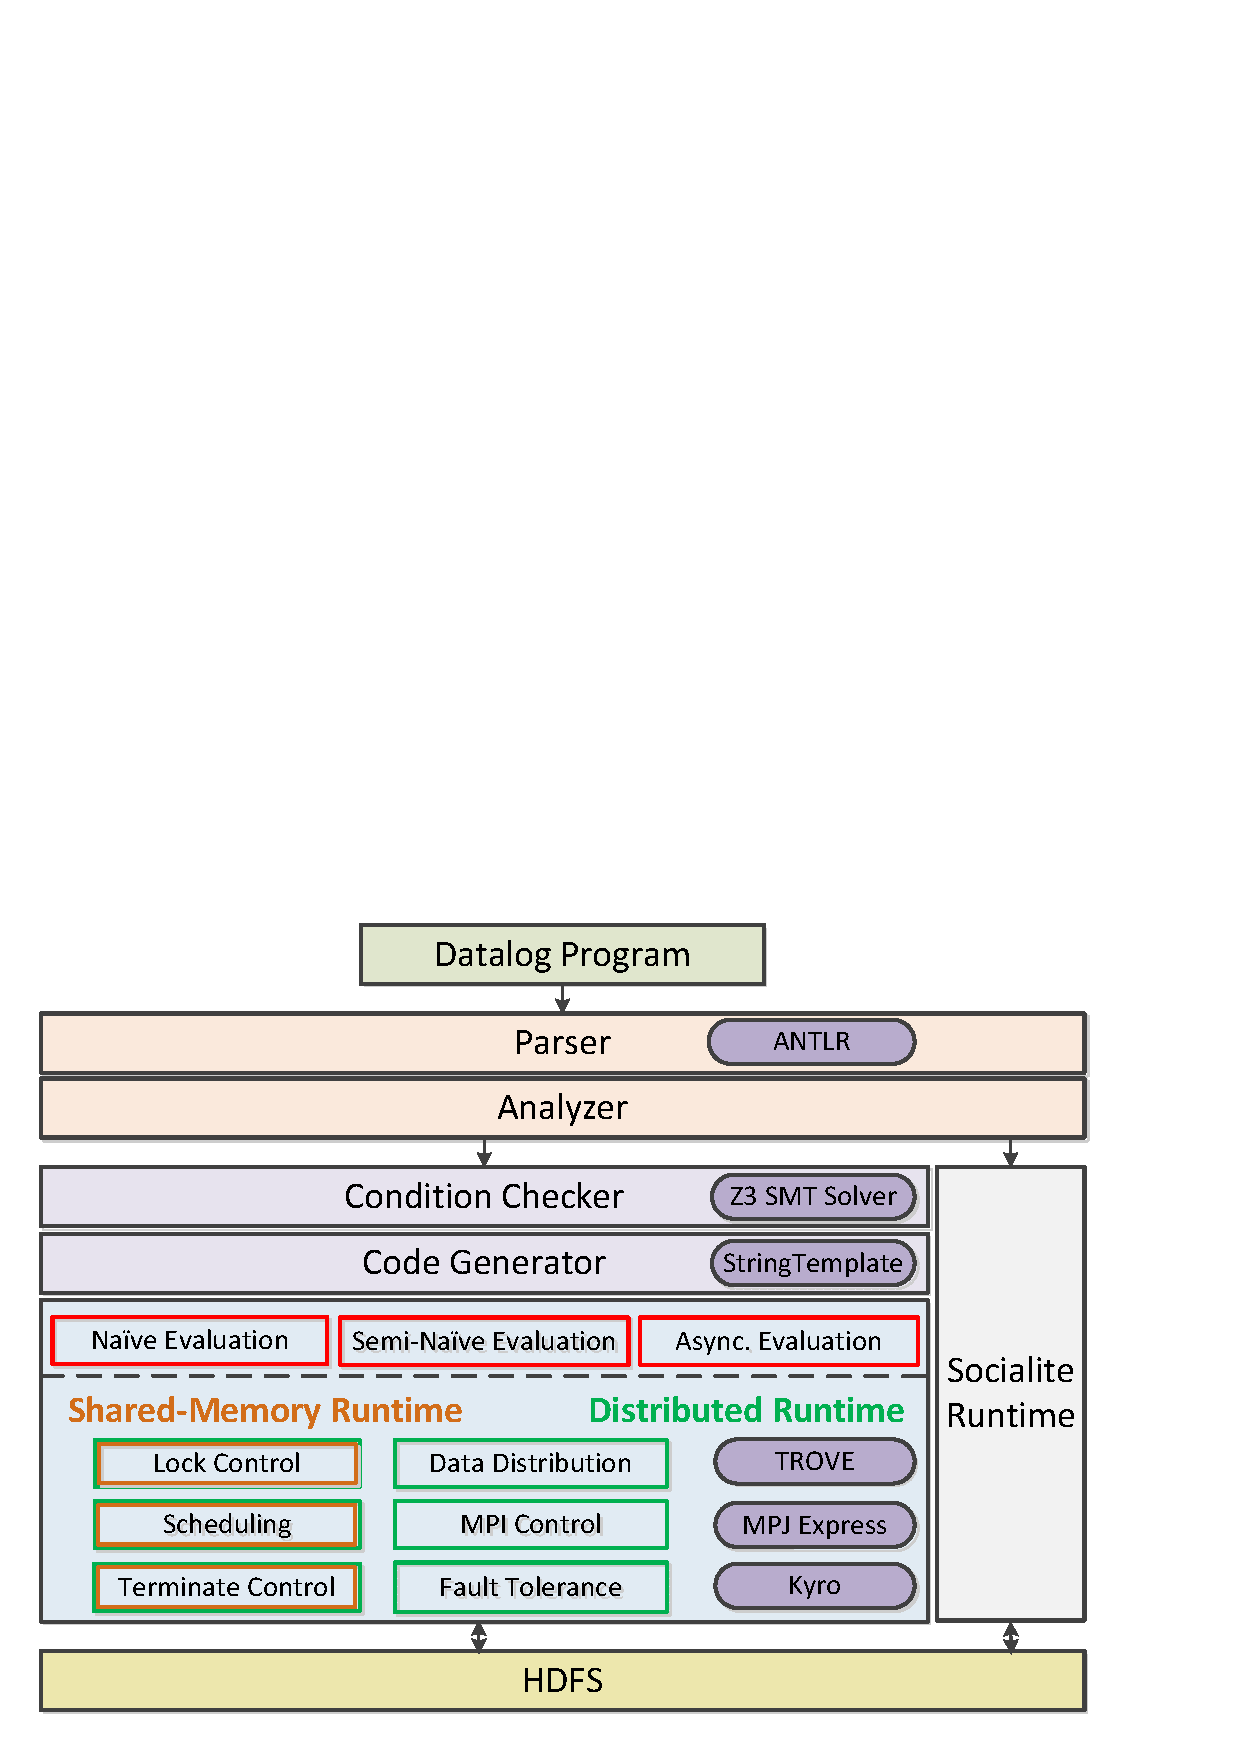
\includegraphics[width=3.2in]{fig/overview}
  \vspace{-0.1in}
  \caption{A3Log overview}
  \label{fig:overview}
  \vspace{-0.2in}
\end{figure}

A3Log is implemented using Java and contains several components as shown in Fig. \ref{fig:overview}. The \textbf{Parser} parses user's Datalog program into an abstract syntax tree (AST) by using ANTLR \cite{antlr}. The \textbf{Analyzer} traverses the AST to performs syntactic and semantic analysis, identifies the recursive rule, and analyzes the aggregate operation $g$ and non-aggregate operation $f$. If the program is a recursive program, it will be further processed by our system, otherwise it will be executed by the Socialite runtime engine \cite{Lam:2013:SDE:2510649.2511289,Seo:2013:DSD:2556549.2556572}. Given the $f$ and $g$ operations retrieved by the Analyzer, the \textbf{Condition Checker} relies on Z3 SMT Solver \cite{DeMoura:2008:ZES:1792734.1792766,z3} to verify the conditions and automatically chooses the appropriate evaluation technique. The \textbf{Code Generator} provides a series of code templates for generating the share-memory runtime code and distributed runtime code, where we use StringTemplate \cite{stringtemplate} to generate source code. Then, the recursive program will be executed by our execution engine (Sec. \ref{sec:system:runtime}). A3Log provides both \textbf{Shared-Memory Runtime Engine} and \textbf{Distributed Runtime Engine}. The shared-memory runtime and distributed runtime share several functionalities, including lock control, scheduling, termination check. The distributed runtime additionally supports data distribution, MPI control, and fault tolerance. We use TROVE \cite{trove} for high performance container operations which are frequently used due to our key table structure, use MPJ Express \cite{mpich} for MPI communication, and use Kryo \cite{kryo} for efficient serialization and deserialization. As implemented in Socialite, A3Log also relies on HDFS to store data and to checkpoint intermediate computation state.

\subsection{Datalog and Extension}
\label{sec:system:datalog}

A Datalog program is a set of rules. A \emph{rule} \texttt{r} has the form $h\leftarrow b_1,\ldots,b_n$, where $h$ is the \emph{head} and $b_1,\ldots,b_n$ is the \emph{body}. The comma separating literals in a body is a logical conjunction (AND). $h$ and $b_i$ can be with the form $p_i(t_1,\ldots,t_j)$ where $p_i$ is a \emph{predicate} and $t_1,\ldots,t_j$ are terms which can be \emph{constants}, \emph{variables} or \emph{functions}. For example, the Datalog program for SSSP computation can be written as follows.
%The data associated with abstract predicate is referred to as \emph{fact}.

\begin{verbatim}
Program 1. Single Source Shortest Path
\end{verbatim}
\vspace{-0.1in}
\small
\begin{lstlisting}
r1. sssp(X,$d$)$\leftarrow$ X=1,$d=0$.
r2. sssp(Y,min[$d$])$\leftarrow$ sssp(X,$d1$),edge(X,Y,$d2$),
$d=d1+d2$,sssp(Y,$d$).
\end{lstlisting}
\normalsize

In Program 1, rule \texttt{r1} initializes the predicate \texttt{sssp} by specifying the source node $X=1$ and the shortest distance from source as $d=0$. \texttt{r2} is a recursive rule since it has the \texttt{sssp} predicate in both its head and body. \texttt{r2} will recursively produce \texttt{sssp} fact by joining the old \texttt{sssp} and \texttt{edge}. If there is a path from source to $X$ of length $d_1$ and an edge from $X$ to $Y$ of length $d_2$, there is a path from source to $Y$ with length $d=d_1+d_2$. If there is already a path to $Y$ found before, it should be also considered. Hence, the shortest distance from source to $Y$ is updated by the minimum of these possible distances, i.e., min$[d]$. The recursion will terminate as soon as no shortest distance is updated.

Originally, the Datalog program terminates when no new fact can be found. However, some programs will never stop since it continuously produces ``tiny'' facts. For example, the PageRank computation will continuously update the PageRank scores even though the changes are less and less. In order to help users express more termination conditions, we allow users to specify the termination conditions using aggregations.


\begin{verbatim}
Program 2 PageRank
\end{verbatim}
\vspace{-0.1in}
\small
\begin{lstlisting}
r1. degree(X,count[Y])$\leftarrow$ edge(X,Y).
r2. rank(X,$r$) $\leftarrow$ node(X),$r=1$.
r3. rank(Y,sum[$r$]+0.15) $\leftarrow$ rank(X,$r1$),edge(X,Y),
degree(X,$d$),
$r=0.85\cdot r1/d$,
[sum$[\Delta r]\leq 0.001$].
\end{lstlisting}
\normalsize

In Program 2, we show the Datalog program for PageRank. \texttt{r1} computes the node degrees based on the edge data. \texttt{r2} initializes the predicate \texttt{rank} by specifying all the nodes' ranking scores as a constant 1. \texttt{r3} is a recursive rule that updates the predicate \texttt{rank}. We allow users to specify the terminate conditions in $[\ldots]$ by using different aggregate operations. In this program, the PageRank computation will terminate when the sum of ranking score differences of two continuous recursion results is less than or equal to 0.001.

Besides SSSP and PageRank, we list 11 more example Datalog programs that can be executed asynchronously in the Appendix Sec. \ref{sec:app:example}. These examples cover a wide range of applications, including graph analytics (Program 3, 4, 5, 12), data mining (Program 6, 7, 9, 10), machine learning (Program 8, 11), and HPC (Program 13).

\subsection{Condition Checker}
\label{sec:system:condition}

\begin{figure}[!t]
    \centering
  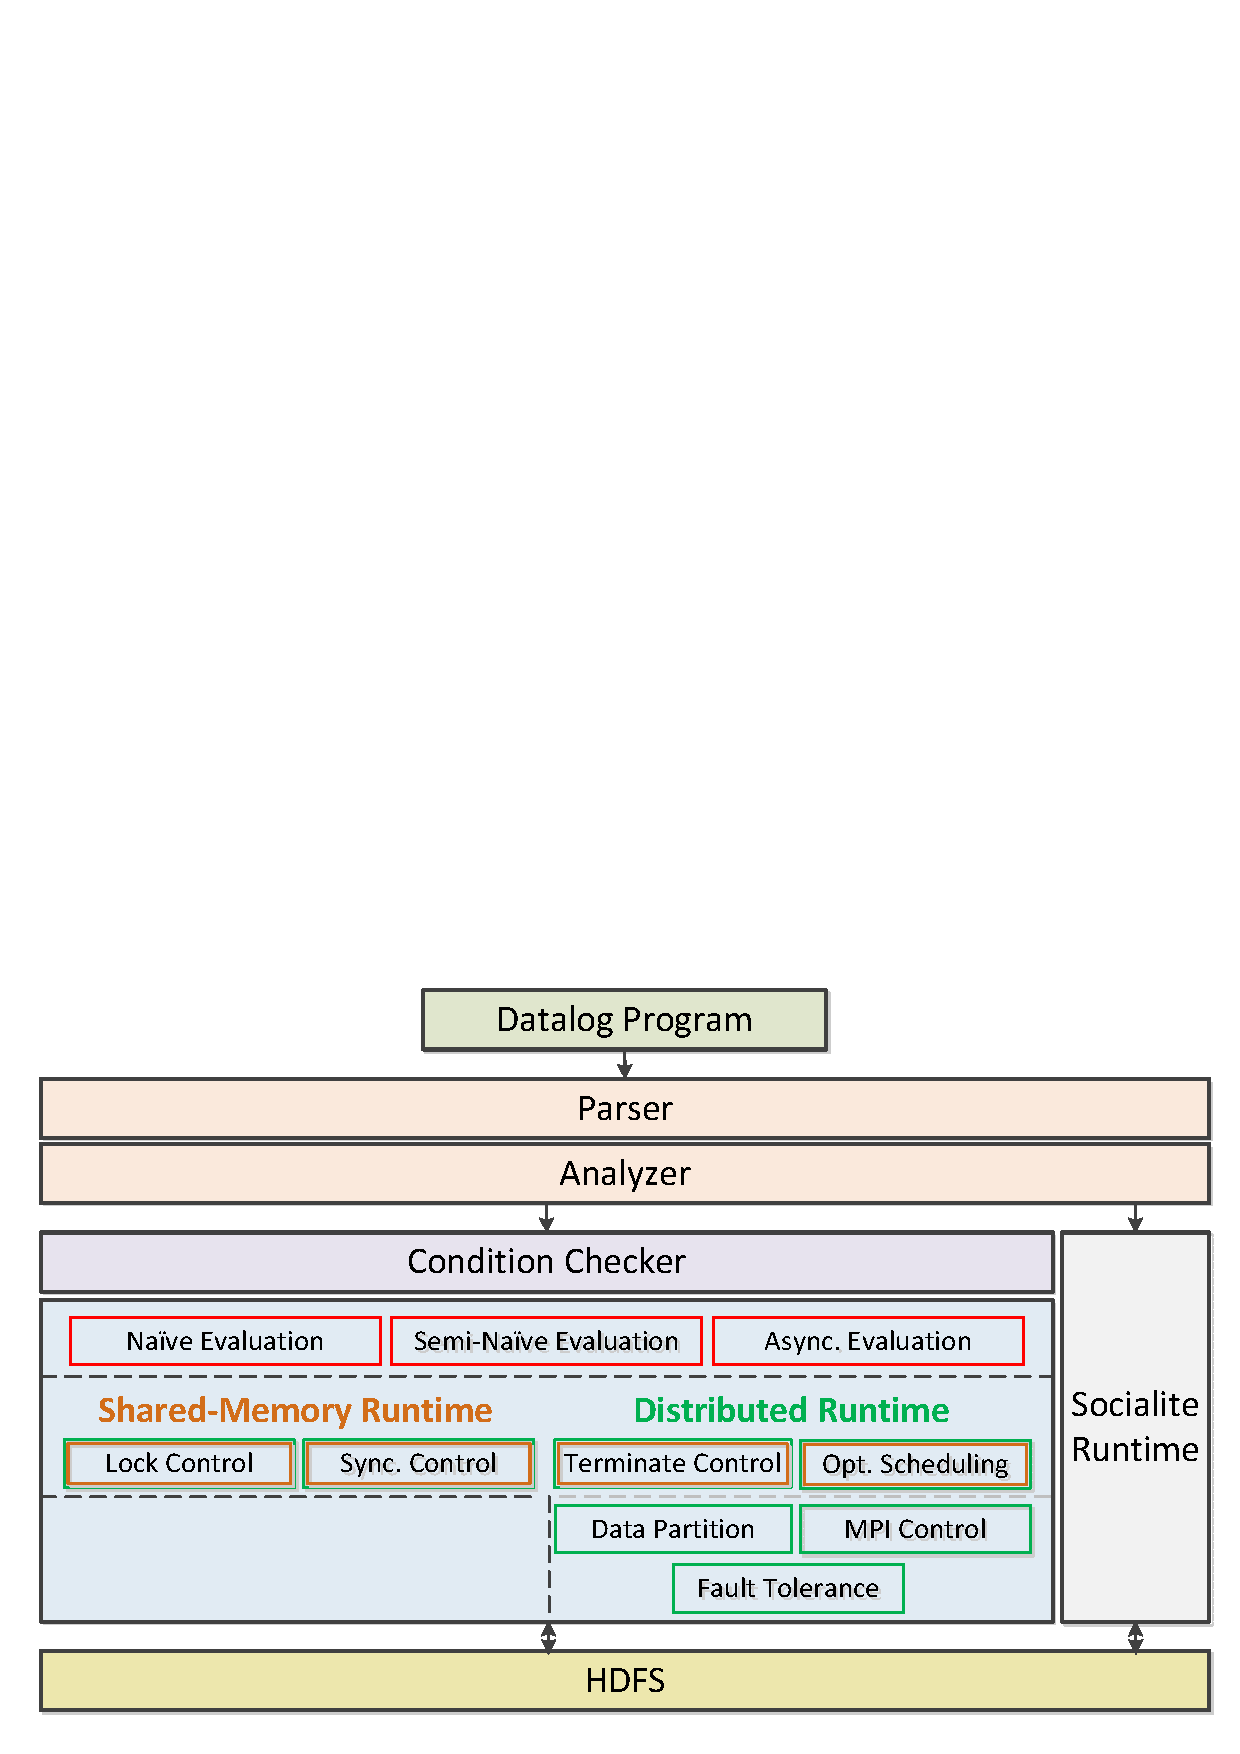
\includegraphics[width=2.8in]{fig/flow}
  \vspace{-0.1in}
  \caption{Condition checking flow chart}
  \label{fig:flow}
  \vspace{-0.2in}
\end{figure}

A3Log is able to automatically verify the conditions for asynchronous aggregation and accordingly selects the appropriate optimization technique according to the satisfiable conditions. The $g$ operation is identified as the update operation in the recursive rule's head predicate, e.g., min[$d$] in SSSP and sum[$r$]+0.15 in PageRank where [$d$] and [$r$] are the inputs, respectively. The $f$ operation is identified as the computation in the recursive rule's certain body predicate that updates the input variables of $g$ operation, e.g., $d=d1+d2$ in SSSP and $r=0.85\cdot r1/d$ in PageRank. The input variable of $f$ operation is the variable that appears in the recursive predicate, e.g., $d1$ in \texttt{sssp(X,$d1$)} and $r1$ in \texttt{rank(X,$r1$)}.

There are two techniques for executing recursive Datalog programs. The first is \emph{\textbf{Naive Evaluation}}. For instance, in Program 1, the recursive rule \texttt{r2} will be repeatedly evaluated. The \texttt{edge} facts keep being joined with the \texttt{sssp} facts discovered so far in each iteration, until no new fact is produced. This approach will inefficiently re-produce known facts in every iteration. To address this inefficiency issue, the \emph{\textbf{Semi-Naive Evaluation}} for recursive programs with aggregation was proposed \cite{Lam:2013:SDE:2510649.2511289,Wang:2015:AFR:2824032.2824052}, which is efficient and produces no duplicates. However, the semi-naive evaluation requires the program to be set-containment monotonic in order to guarantee the correctness. This is the same as the monotonizability condition that we have defined in Theorem \ref{th:monotone}. Therefore, as long as the program satisfies monotonizability condition or can be converted to be monotonic according to Theorem \ref{th:convert}, it can be executed with semi-naive evaluation. Furthermore, we propose \emph{\textbf{asynchronous evaluation}} as a yet another optimization technique, which allows asynchronous aggregation. We provide the sufficient conditions for asynchronous aggregation in Theorem \ref{th:async}. The prerequisite for asynchronous aggregation is the monotonic condition. Asynchronous evaluation is possible only when the recursive program is monotonic and satisfies order independent condition.

Condition Checker first translates the $f$ and $g$ operations into Z3 \cite{DeMoura:2008:ZES:1792734.1792766} satisfiability formulas (see Sec. \ref{sec:async:autoasync}). By applying $f$ and $g$ to the built-in condition checking templates, the Z3 SMT olver will answer satisfiable, unsatisfiable, or unknown. Following the condition checking flow as shown in Fig. \ref{fig:flow}, our system can automatically select the appropriate evaluation technique.

\subsection{Key Data Structure: AsyncTable}
\label{sec:system:data}

Before launching the recursive computation, the key table structure, AsyncTable, should be first prepared. AsyncTable maintains the computation states, which are initialized based on user's Datalog program and keeps being updated during the whole recursive computation process.

\begin{figure}[!t]
    \centering
  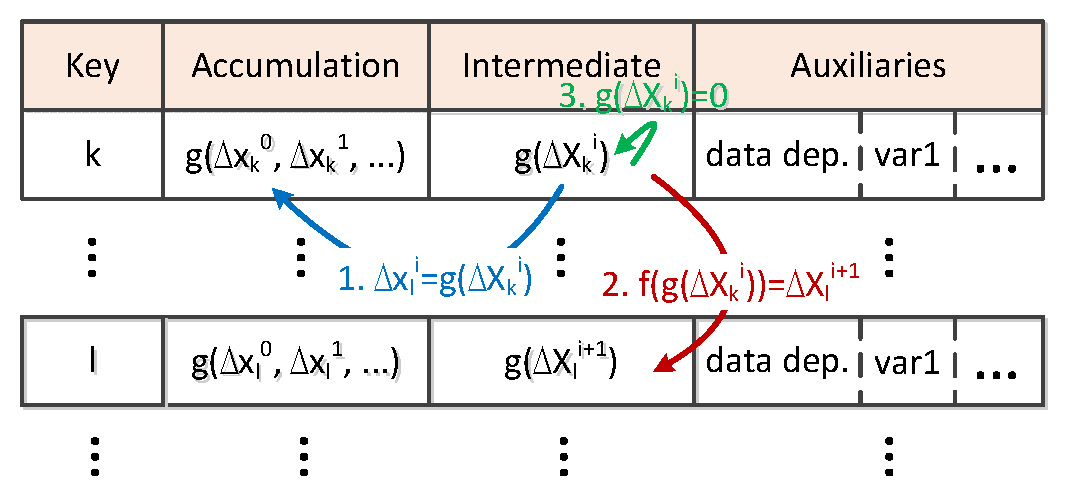
\includegraphics[width=3.2in]{fig/asynctable}
  \vspace{-0.1in}
  \caption{AsyncTable update}
  \label{fig:asynctable}
  \vspace{-0.2in}
\end{figure}


\noindent\textbf{AsyncTable Design}
As shown in Fig. \ref{fig:asynctable}, the AsyncTable contains several columns. The main key column and accumulation column store the result key-value pairs. The main key entries index the table. The accumulation column entry monotonically aggregates the intermediate results and maintains $g(\Delta x^0,\Delta x^1,\ldots)$. The accumulative property of $g$ operation makes it possible to use a single column to maintain all the intermediate results. The intermediate column entry stores the temporary aggregation results $g(\Delta X^k)$ which will be used to generate future intermediate results by applying $f$ operation. The auxiliary columns store the data which might be used by the $f$ or $g$ operation, e.g., outgoing neighbors set in SSSP and the node degree value in PageRank. The accumulation column entries and intermediate column entries are volatile, which maintain the computation states and keep being updated during the computation, while the other column entries are fixed after initialization. The AsyncTable is sharded for parallel processing. Each shard contains a number of rows and is assigned to a compute thread or placed on a distributed worker machine.

\noindent\textbf{AsyncTable Initialization}
The AsyncTable is initialized according to user's program. The recursive rule head contains the main key and accumulation column's information. For example in SSSP, the main key column entries are initialized with the node ids. The accumulation column is initialized with the identity element \textbf{0} w.r.t $g$, e.g., MAX in SSSP. The intermediate column is initialized in terms of the non-recursive rule \texttt{r1}, i.e., 0 for the source node and MAX for other nodes. The auxiliary data dependency column is identified as the rule body predicate that describes the relationship between main keys, e.g., \texttt{edge(X,Y,d2)}. The auxiliary variable column entries can be identified as the joined results between rule body predicates, e.g., the degree information \texttt{d} in PageRank.

A few additional facts should be noticed: 1) It is possible that two or more items are identified as the main key (see Program 4, 5, and 12 in Appendix Sec. \ref{sec:app:example}); 2) The AsyncTable size can be dynamic rather than fixed due to the continuously inserted new rows (see Program 4, 5, 7, and 9); 3) The recursive program can be composed of more than one interdependent rules, which can be reduced to one rule (see Program 9 and 10).

\subsection{Execution Runtime Engine}
\label{sec:system:runtime}

\begin{figure}[!t]
    \centering
  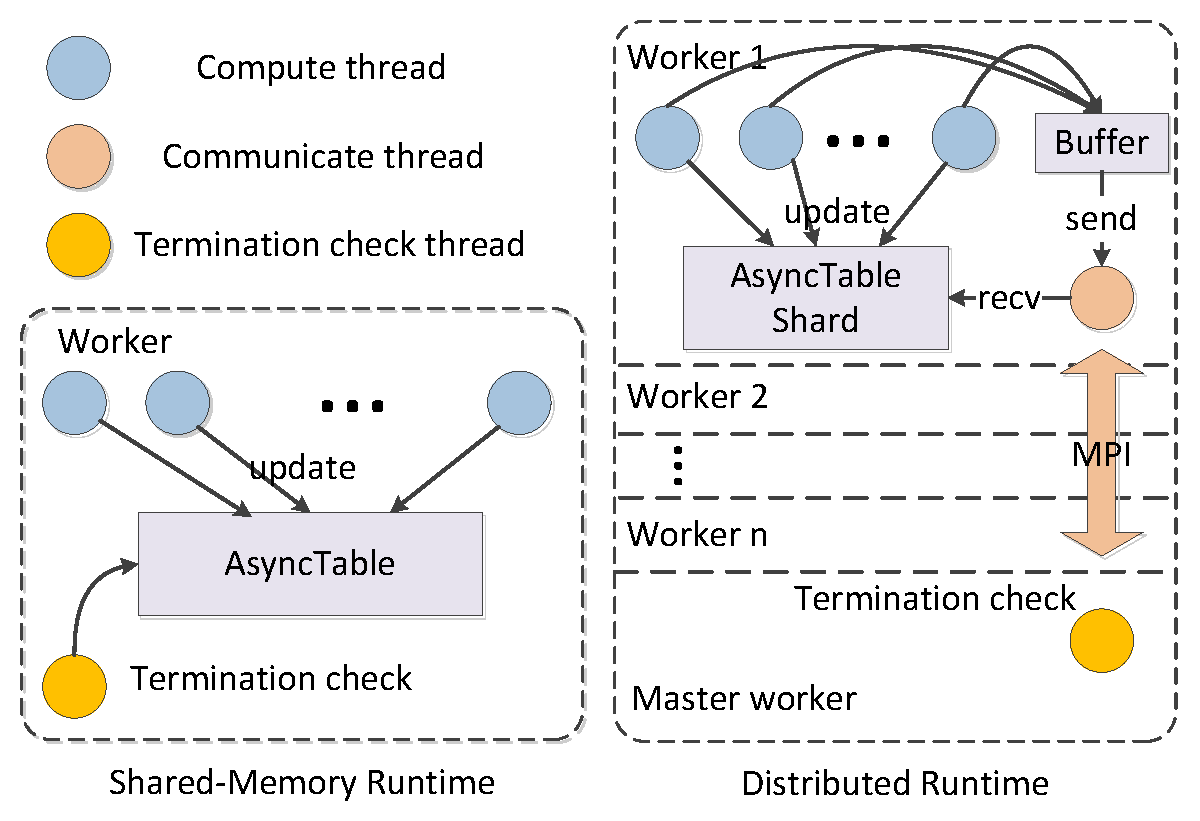
\includegraphics[width=2.9in]{fig/runtime}
  \vspace{-0.1in}
  \caption{Execution Runtime Engine}
  \label{fig:runtime}
  \vspace{-0.1in}
\end{figure}

\noindent\textbf{Overall Architecure}
A3Log provides both shared-memo-ry runtime engine and distributed runtime engine. Fig. \ref{fig:runtime} shows the overall structure. The shared-memory runtime has a simple design. A number of compute threads are created to update the AsyncTable in parallel, and a termination check thread is running separately to check the stop condition. The distributed runtime contains a number of workers and a master worker. Each worker creates a number of compute threads to update the local AsyncTable shard. A communicate thread tackles the remote update. We adopt a send buffer design to control the overhead of frequent communications. The master worker creates a termination check thread to globally check stop condition periodically.


\noindent\textbf{Concurrency Control}
The accumulation column entries and intermediate column entries keep being updated during computation. Specifically, an intermediate column entry is read to update the same row's accumulation column entry (by operation 1 in Fig. \ref{fig:asynctable}) and to update other rows' intermediate column entries (by operation 2 in Fig. \ref{fig:asynctable}), and is reset as \textbf{0} (by operation 3 in Fig. \ref{fig:asynctable}). The reset operation is essential to make result correct, without which the same intermediate result would be redundantly accumulated. These three operations have to be \emph{atomic} according to the definition of accumulated recursive program (Definition \ref{eq:accumasync}). However, an intermediate column entry can be read and written concurrently by multiple threads or multiple workers, which leads to potential consistency problem. In our shared-memory runtime, we use \emph{optimistic} lock to avoid read-write conflicts. In distributed runtime, the consistency problem will happen in the send buffer, which maintains the remote updates. The optimistic lock does not work well since the communicate thread is required to serialize the whole buffer for efficiency and the lock granularity becomes too coarse to result in too many aborts. We employ MVCC (multi-version concurrency control) to address this problem. Specifically, we adopt a double-version design of the send buffer, which serves the compute threads and communicate thread alternatively.


\noindent\textbf{Scheduling}
As discussed in Sec. \ref{sec:async:pri}, the clever scheduling of aggregate operations has the potential of accelerating the convergence of recursive computations. The scheduling should be performed by evaluating the intermediate aggregation result (intermediate column entries in AsyncTable). The top intermediate column entries (in the partial order defined by $g$) should be scheduled. Since the intermediate column entries keep being updated, the top entries should be evaluated frequently. For the sake of reducing scheduling cost, we utilize the sampling technique \cite{Zhang:2011:PDF:2038916.2038929} to approximately obtain the top $N\%$ entries. The scheduling is even more costly in distributed environment. Rather than global scheduling, local scheduling in each worker is preferred.
%The portion ($N\%$) of entries to be scheduled balances the tradeoff between the optimal scheduling benefit and the sorting cost. We will empirically study the effect of $N\%$ in Sec. \ref{sec:expr:schedle}.

\noindent\textbf{Termination Check}
The termination condition might rely on aggregation of either the accumulation column entries or the intermediate column entries. The aggregation is evaluated by the termination check thread without disturbing the compute threads. While in distributed runtime, each worker will report their local aggregation results to the master, where the global termination check thread determines whether to stop by evaluating the global aggregation result. Note that, there is no iteration's conception in asynchronous aggregation, so we have to check the termination condition every other period of time rather than every other iteration.

\noindent\textbf{Fault Tolerance}
For large scale operations that involve many machines for a substantial amount of time, it is also important to provide fault tolerance support. A3Log relies on Socialite's fault tolerance scheme \cite{Seo:2013:DSD:2556549.2556572}. The intermediate computation states are checkpointed occasionally on HDFS and restorable as needed. If one or more workers fail, the intermediate states are restored from the latest checkpoint and the evaluation is resumed from that point.

\section{Performance Evaluation}
\label{sec:expr}

We empirically evaluate A3Log on Amazon EC2. We will show the comparison results with other systems, with different algorithms, and with different datasets. More experimental results can be found in Appendix Sec. \ref{sec:app:expr}, including scaling performance and effectiveness of aggregations.



\subsection{Comparison to Other Systems}
\label{sec:expr:othersystems}

\noindent\textbf{Competitors}
A3Log is compared with four state-of-the-art parallel/distributed frameworks. \textbf{SociaLite} \cite{Lam:2013:SDE:2510649.2511289,Seo:2013:DSD:2556549.2556572} is a Datalog implementation for social network analysis. \textbf{Myria} \cite{Halperin:2014:DMB:2588555.2594530,Wang:2015:AFR:2824032.2824052} supports Datalog asynchronous evaluation. Both SociaLite and Myria support monotonic aggregation inside recursion. \textbf{GraphLab} \cite{Low:2012:DGF:2212351.2212354} is a graph-based parallel/distributed engine supporting asynchronous iteration. \textbf{Maiter} \cite{maiter} supports delta-based accumulative iterative computation (similar to monotonic aggregation) which can be executed asynchronously. All these systems are configured with their default parameters. Myria, GraphLab, and Maiter are configured to run with asynchronous model unless particularly mentioned. The runtime results are the execution time excluding data loading time, and each is a mean of two runs.

\noindent\textbf{Algorithms and Datasets}
We compare A3Log with other systems in the context of three algorithms, including SSSP (Program 1), PageRank (Program 2), and Connected Components (CC, Program 3). These three algorithms are all supported by these systems. For SSSP and CC, the computations terminate as soon as no new update is found. For PageRank in A3Log and Maiter, which has no notion of iterations, the computation terminates when the sum of difference to the theoretical convergence point \cite{Zhang:2011:PDF:2038916.2038929} is less than $10^{-4}$ (see Appendix Sec. \ref{sec:expr:aggregations}), based on which we know the number of iterations that is required to reach the same point (42 iterations) \cite{Zhang:2011:PDF:2038916.2038929}. Socialite and Myria (Myria does not support asynchronous PageRank) are set to run 42 iterations. GraphLab terminates after the PageRank value of every vertex changes by less than a user-specified threshold $\epsilon$ between two consecutive executions of that vertex. These algorithms are performed on a large graph dataset ClueWeb09 \cite{clueweb}. In order to finish the experiments in a reasonable time, we truncate the original dataset into a smaller ClueWeb20M dataset with 20,000,000 nodes, 243,063,334 edges, and 3.8GB size. Since ClueWeb is an unweighted graph, we assign a random weight to each edge for SSSP computation.

\begin{figure}[!t]
	\vspace{-0.1in}
	\centering
	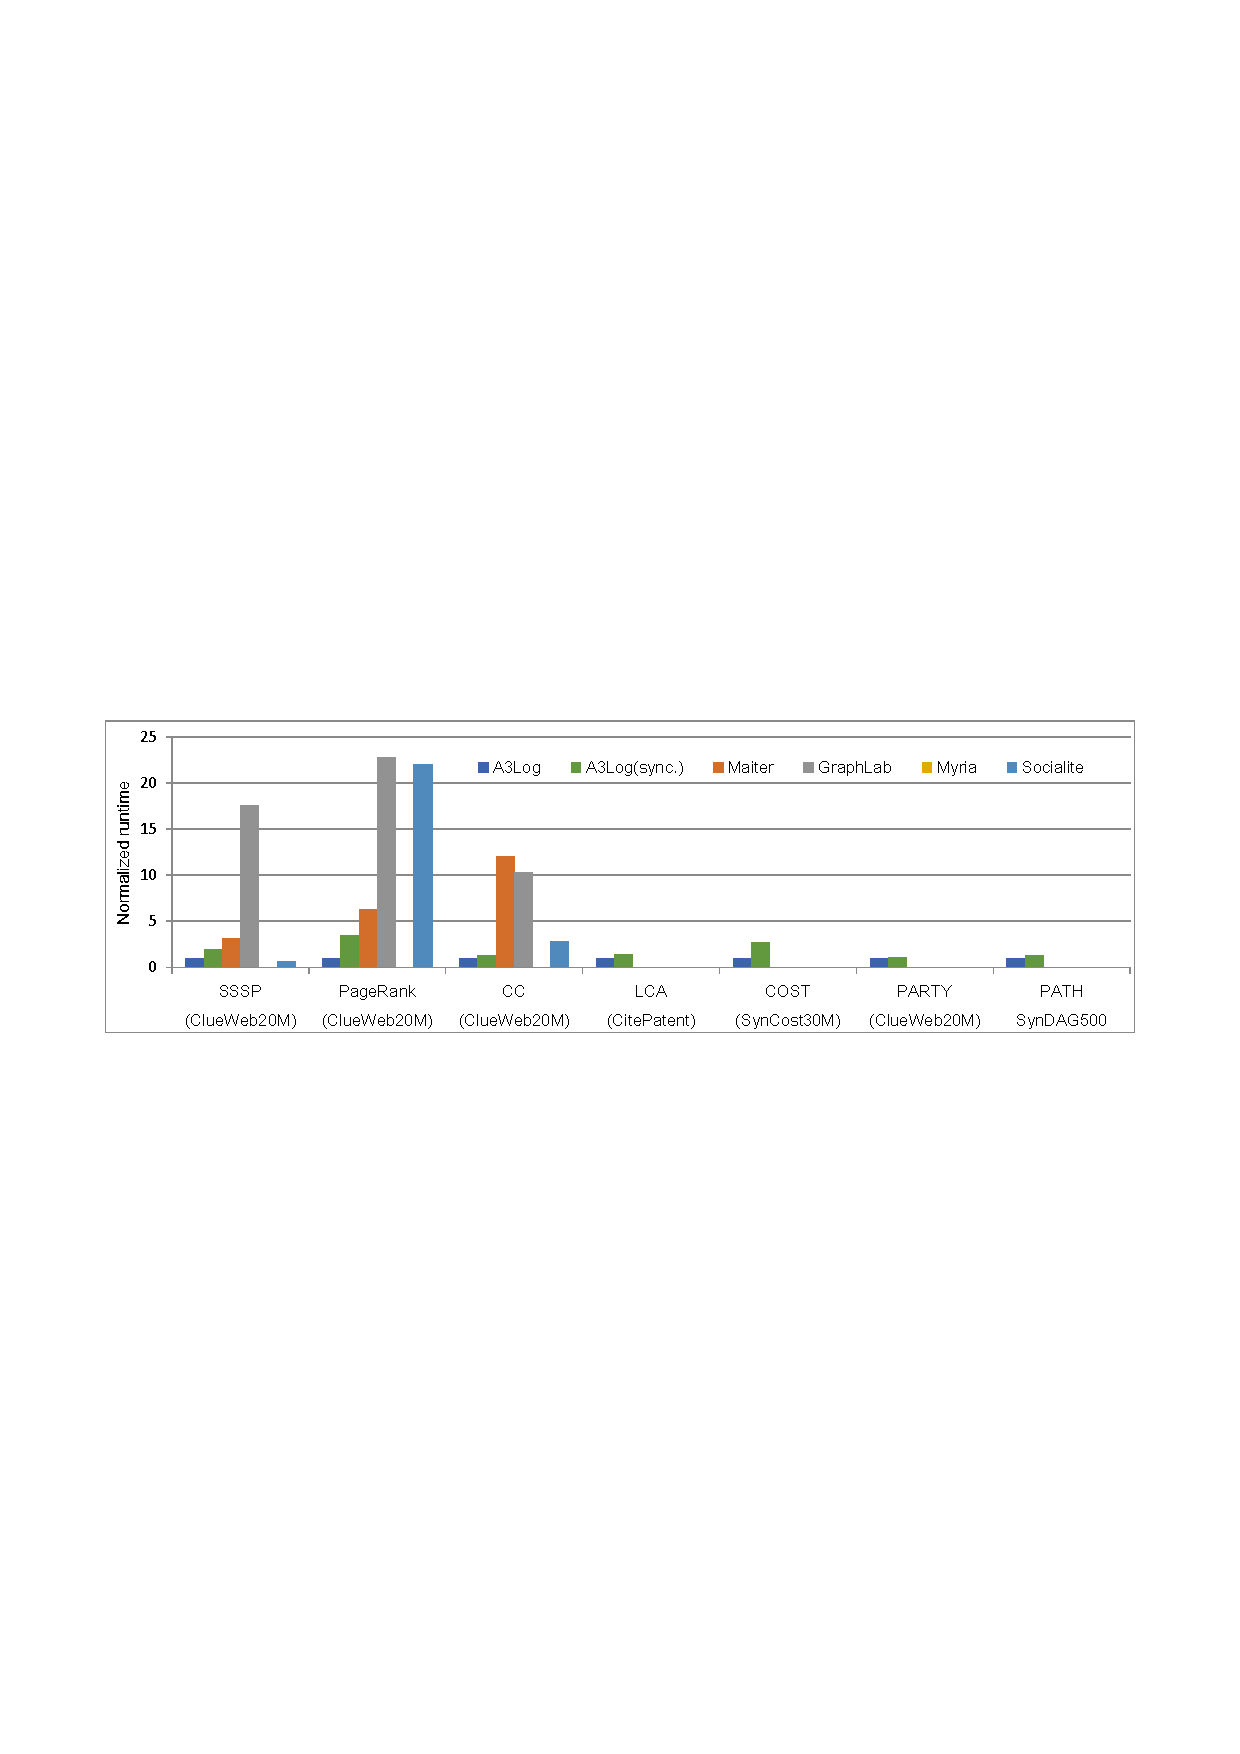
\includegraphics[width=3in]{fig/single-result}
	\vspace{-0.1in}
	\caption{Performance comparison with other systems (many-core environment)}
	\label{fig:single-result}
	\vspace{0.0in}
\end{figure}

In the shared-memory experiment, we run all the systems on an r3.8xlarge EC2 instance with 32 vCPUs and 244GB memory. We configured all these systems with 32 threads. The normalized runtime results. In general, A3Log outperforms all the competitors. For the PageRank computation, A3Log achieves 22.8X speedup over GraphLab, 22X speedup over Socialite, 6X speedup over Maiter, and much more speedup over Myria\footnote{The runtime results of Myria may be wrong because they are all unexpected long, say 135 times longer for PageRank and 321 times longer for SSSP than A3Log. We are contacting with Myria authors to fix it but cannot find the problem before the submission.} are shown in Fig. \ref{fig:single-result}. There is an exception for SSSP computation. Socialite is 1.6X faster than A3Log. This may be due to their \emph{prioritization} optimization, which is similar to our scheduling technique that leads to Dijkstra algorithm.

\begin{figure}[!t]
	\vspace{0.0in}
	\centering
	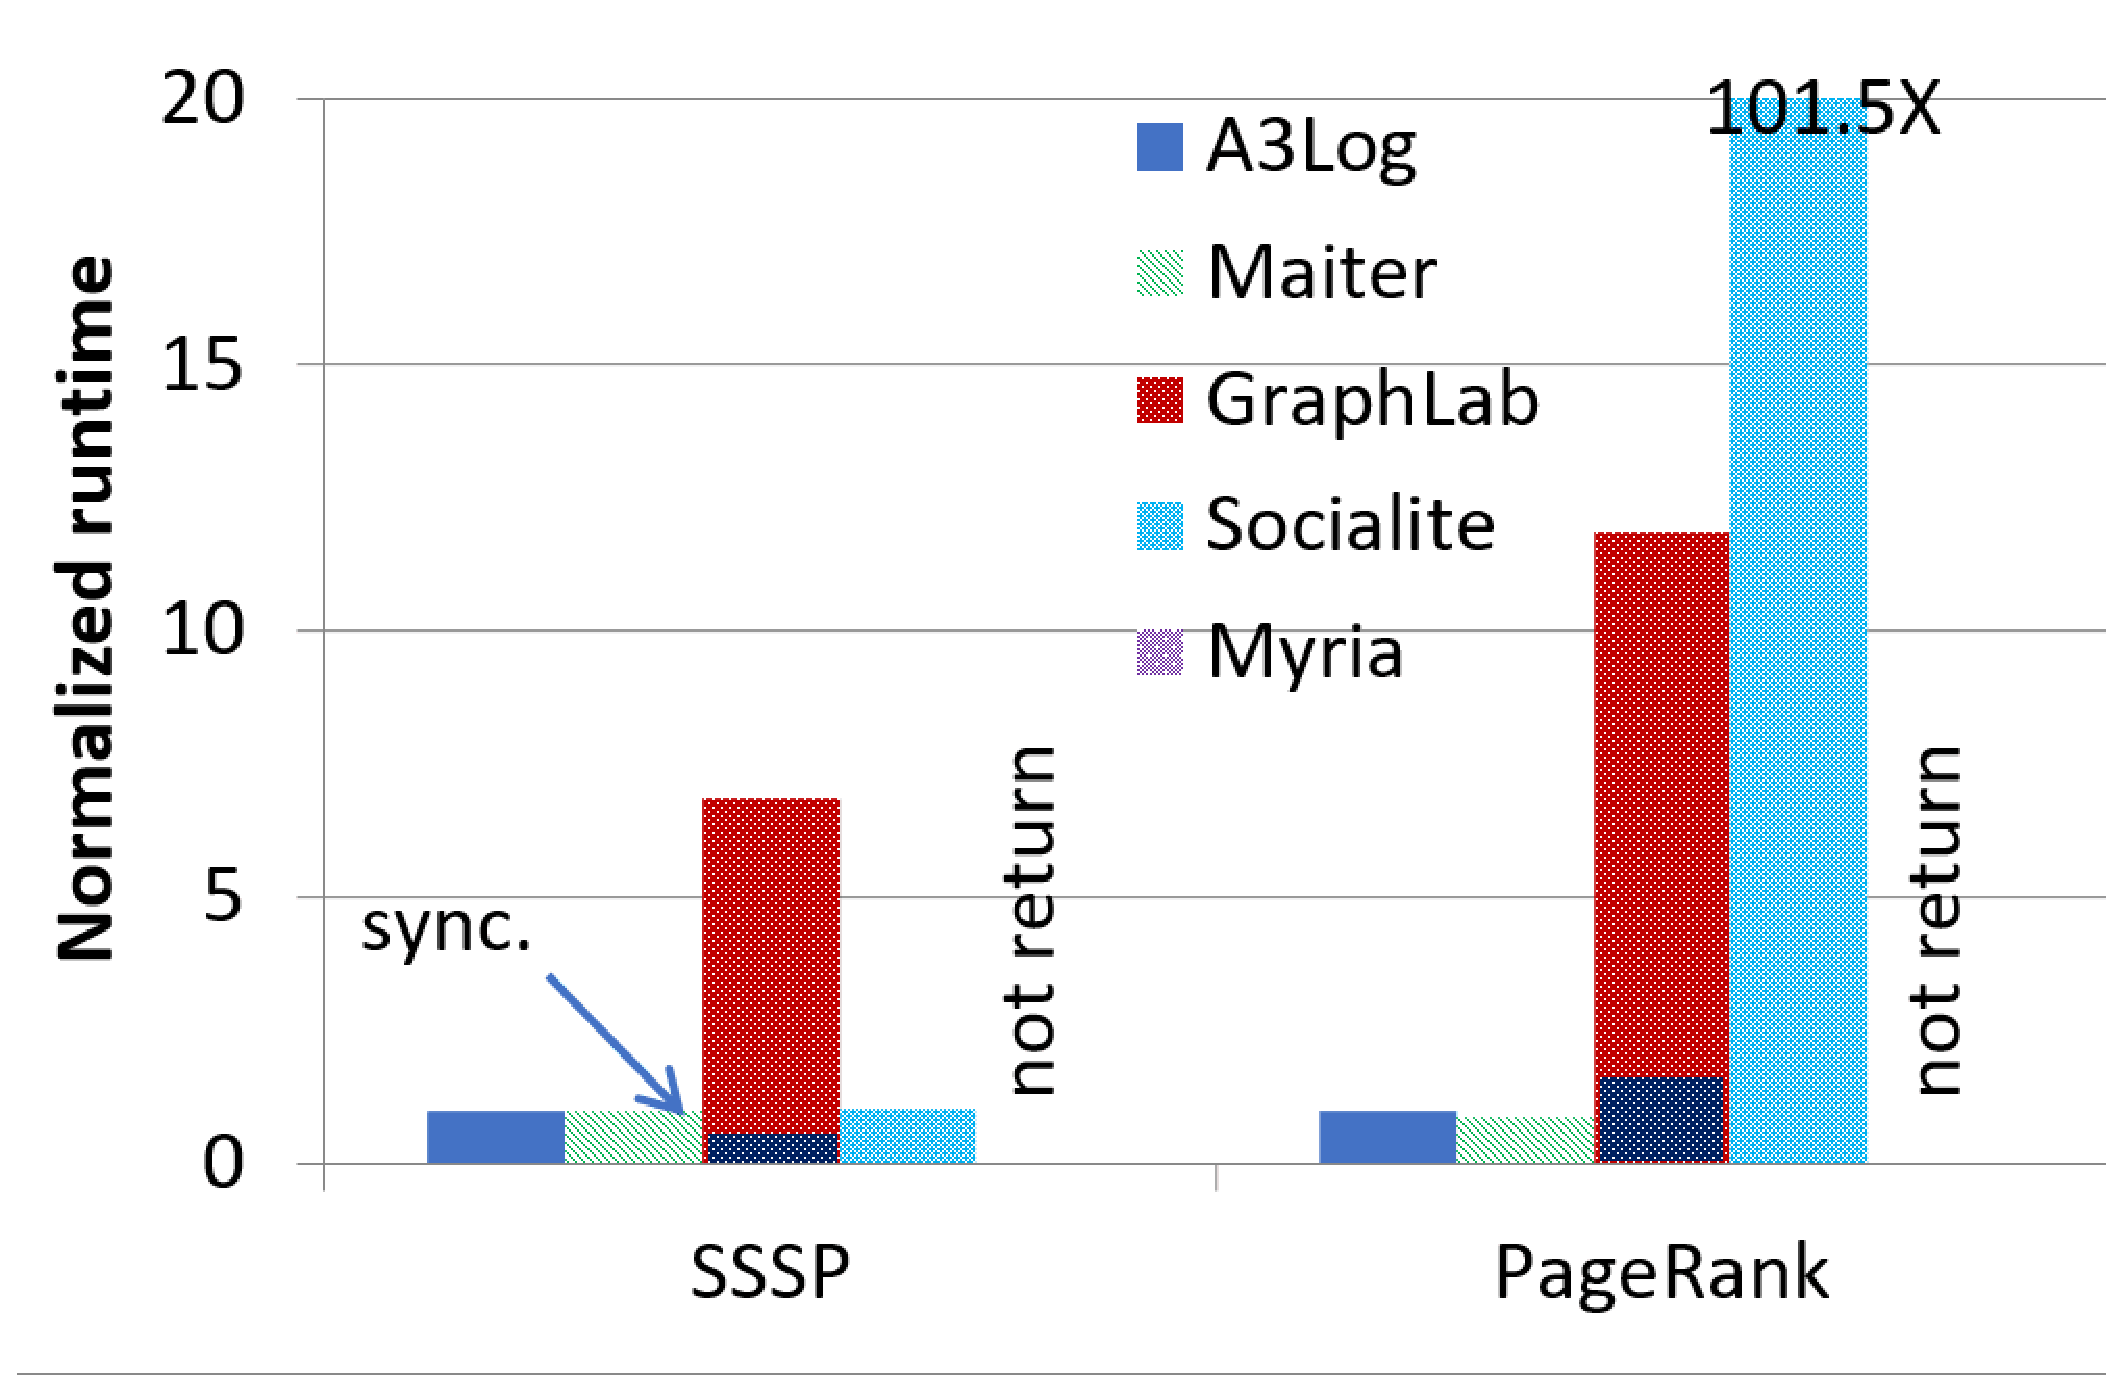
\includegraphics[width=2.4in]{fig/dist-result}
	\vspace{-0.1in}
	\caption{Performance comparison with other systems (distributed environment)}
	\label{fig:dist-result}
	\vspace{-0.2in}
\end{figure}

In the distributed experiment, we deploy all the systems on an EC2 cluster with 64 c4.2xlarge EC2 instances, each with 8 vCPUs and 15GB memory. The network bandwidth between instance workers is 10Gb/s\footnote{The network specification does not clearly describe the bandwidth but is only classified as \emph{High}, which is estimated as 10Gb/s.}. We configured all these systems with 8 threads for each worker. The normalized runtime results of SSSP and PageRank are shown in Fig. \ref{fig:dist-result}. A3Log outperforms GraphLab and Socialite on PageRank computation. The synchronous version of GraphLab performs much better than asynchronous GraphLab, which is due to its costly distributed locking \cite{Han:2015:GUB:2777598.2777604,Low:2012:DGF:2212351.2212354}. Socialite performs SSSP faster. The distributed Myria runs unexpected long without returning results, say 9 hours for PageRank and did not return. The performance of A3Log and Maiter is comparable on these two applications. The reason why A3Log does not show significant better performance in distributed environment is because of the expensive communication overhead. The communication module relies on a pure Java implementation of MPI, MPJ express \cite{mpich}, which shows about 10 times lower performance than native C implementation of Open MPI \cite{mpjperformance}. We adopt MPJ for its good compatibility but at the expense of performance. We are implementing an alternative distributed runtime based on Open MPI \cite{openmpi}.

\subsection{Performance Gain Analysis}
\label{sec:expr:optimizations}

\begin{figure}[!t]
\vspace{-0.1in}
	\centering
	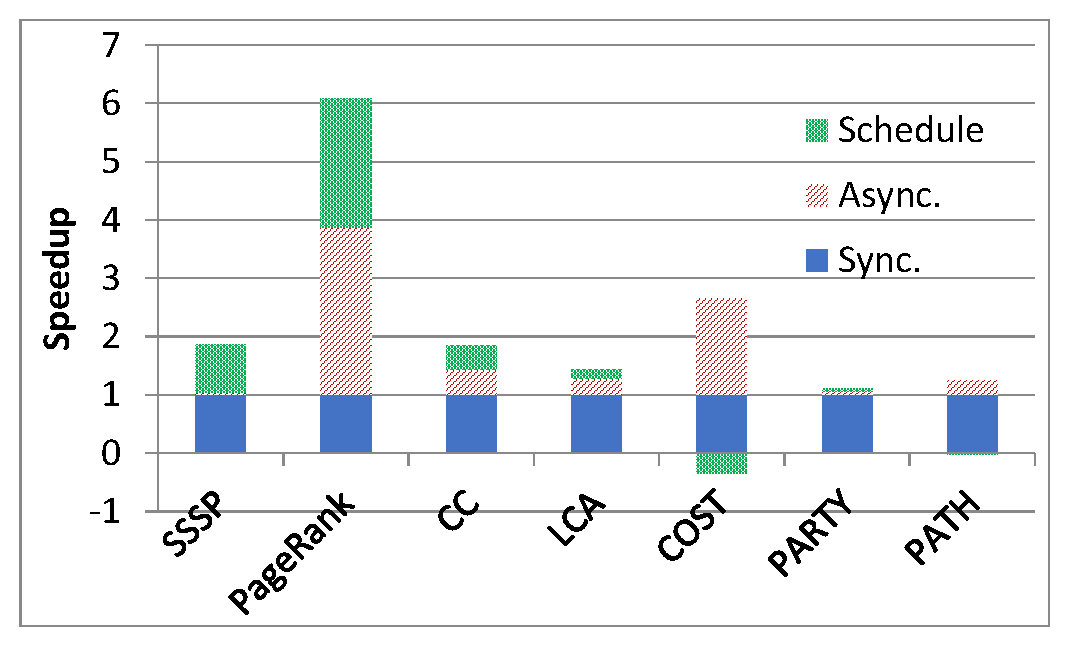
\includegraphics[width=2.8in]{fig/single-optimize}
	\caption{Performance gain analysis}
	\label{fig:single-optimize}
	\vspace{-0.0in}
\end{figure}

\begin{figure}[!t]
	\centering
	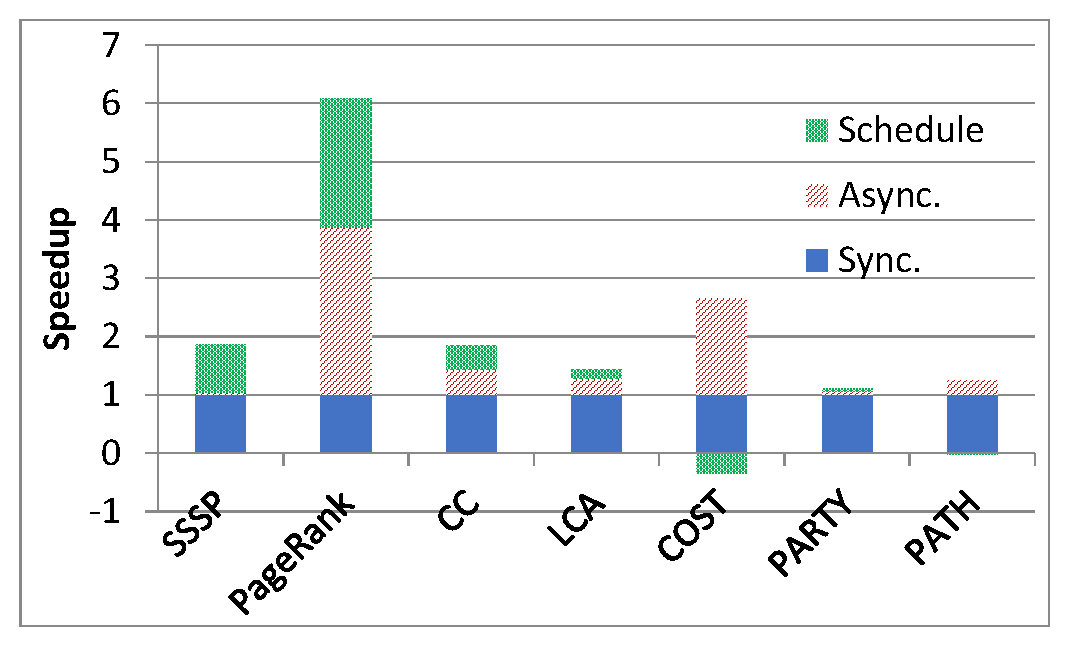
\includegraphics[width=2.8in]{fig/single-optimize}
	\caption{Performance gain analysis}
	\label{fig:single-optimize}
	\vspace{-0.2in}
\end{figure}

\begin{table*}[!t]
	%\vspace{-0.1in}
	\caption{Performance when varying workloads (shared-memory runtime, $d$ is diameter, $e$ is powerlaw exponent)}
	\vspace{-0.1in}
	\label{tab:wrokload}
	\centering
	\small
	\begin{tabular}{c|c|c|c|c|c|c|c|c|c|c|c}
		\hline
		\multirow{2}{*}{\textbf{Dataset}} & \multirow{2}{*}{\tabincell{c}{\textbf{Nodes}}} & \multirow{2}{*}{\tabincell{c}{\textbf{Edges}}} & \multirow{2}{*}{\tabincell{c}{\textbf{Graph}\\ \textbf{type}}} & \multirow{2}{*}{\tabincell{c}{\textbf{$d$}}}& \multirow{2}{*}{\tabincell{c}{\textbf{$e$}}} & \multicolumn{3}{|c}{\textbf{SSSP}} & \multicolumn{3}{|c}{\textbf{PageRank}} \\
		\cline{7-12}
		&  & & & & & \textbf{Sync.} & \textbf{Async.} & \footnotesize{\textbf{Speedup}} & \textbf{Sync.} & \textbf{Async.} & \footnotesize{\textbf{Speedup}}\\
		\hline\hline
		\textbf{Actor} & 382,219 & 33,115,812 & \footnotesize{collaborate} & 13 & 2.131 & 34.62s & 1.54s & 22.44X & 63.62s & 7.03s & 9.05X \\
		\hline
		\textbf{Amazon} & 403,394 & 3,387,388 & \footnotesize{co-purchase} & 25 & 3.151 & 79.18s & 1.55s & 51.05X & 53.77s & 1.02s & 52.9X \\
		\hline
		\textbf{arXiv} & 28,093 & 4,596,803 & co-author & 9 & 1.731 & 19.7s & 1.51s & 13.03X & 53.2s & 1.01s & 52.7X \\
		\hline
		\textbf{DBLP} & 1,314,050 & 18,986,618 & co-author & 24 & 3.221 & 55.38s & 3.18s & 17.41X & 89.76s & 5.06s & 17.75X \\
		\hline
		\textbf{Flicker} & 2,302,925 & 33,140,017 & social & 23 & 1.711 & 38.3s & 3.95s & 9.71X & 84.24s & 24.2s & 3.48X \\
		\hline
		\textbf{Livejournal} & 5,204,176 & 49,174,464 & social & 23 & 1.537 & 57.26s & 9.41s & 6.08X & 111.09s & 49.43s & \textcolor{blue}{\textbf{2.25X}} \\
		\hline
		\textbf{Orkut} & 3,072,441 & 117,184,899 & social & 10 & 1.272 & 58.99s & 14.07s & \textcolor{blue}{\textbf{4.19X}} & 187.74s & 16.18s & 11.6X \\
		\hline
		\textbf{Patent-US} & 3,774,768 & 16,518,947 & citation & 26 & 4.001 & 66.83s & 3.21s & 20.8X & 68.06s & 6.11s & 11.15X \\
		\hline
		\textbf{Prosper} & 89,269 & 3,394,979 & loan & 8 & 2.191 & 37.75s & 1.51s & 24.93X & 52.61s & 1.02s & 51.58X \\
		\hline
		\textbf{RoadCA} & 1,965,206 & 2,766,607 & road net & 865 & 8.991 & 140.43s & 1.55s & 90.31X & 57.06s & 1.03s & \textcolor{red}{\textbf{55.59X}} \\
		\hline
		\textbf{RoadTX} & 1,379,917 & 1,921,660 & road net & 1064 & 8.901 & 137.2s & 1.55s & 88.4X & 54.49s & 1.02s & 53.63X \\
		\hline
		\textbf{Skitter} & 1,696,415 & 11,095,298 & Internet & 31 & 2.291 & 31.09s & 1.55s & 20.01X & 59.51s & 3.04s & 19.56X \\
		\hline
		\textbf{soc-LiveJ} & 4,847,571 & 68,475,391 & social & 20 & 2.651 & 67.2s & 11.2s & 6X & 113.51s & 39.2s & 2.9X \\
		\hline
		\textbf{soc-Pokec} & 1,632,803 & 30,622,564 & social & 14 & 3.081 & 53.85s & 4.81s & 11.19X & 76.83s & 15.1s & 5.09X \\
		\hline
		\textbf{TREC} & 1,601,787 & 8,063,026 & web & 112 & 2.231 & 130.84s & 1.6s & 81.62X & 55.29s & 2.03s & 27.23X \\
		\hline
		\textbf{\footnotesize{web-BerkStan}} & 685,230 & 7,600,595 & web & 208 & 2.601 & 692.08s & 3.1s & \textcolor{red}{\textbf{222.82X}} & 54.13s & 2.02s & 26.76X \\
		\hline
		\textbf{web-Google} & 875,713 & 5,105,039 & web & 24 & 2.731 & 70.8s & 1.59s & 44.64X & 54.24s & 2.03s & 26.67X \\
		\hline
		\textbf{Wiki-Talk} & 2,987,535 & 24,981,163 & \footnotesize{communicate} & 9 & 1.811 & 23.81s & 3.1s & 7.68X & 83.57s & 28.27s & 2.96X \\
		\hline
		\textbf{Youtube-u} & 3,223,589  & 9,375,374 & social & 31 & 2.211 & 30.6s & 2.43s & 12.6X & 65.91s & 5.08s & 12.96X \\
		\hline
		\textbf{\footnotesize{Zhishi-Baidu}} & 2,141,300 & 17,794,839 & web & 20 & 2.291 & 49.19s & 3.29s & 14.96X & 66.72s & 8.09s & 8.25X\\
		\hline
	\end{tabular}
	\vspace{-0.1in}
\end{table*}


In order to analyze the factors for performance improvement and eliminate the interference from system implementation factors, we also implement a synchronous version of A3Log, which uses synchronous semi-naive evaluation (i.e., synchronous accumulated recursive programs). In addition, we turn off the scheduling then it shows the performance ahieved by pure asynchronous aggregation.

\noindent\textbf{Algorithms and Datasets}
We test more algorithms to see the effect variations on different workloads, including Least Common Ancestor (LCA, Program 6), ``What is the cost of each part?'' (COST, Program 7), ``Who will come to the party?'' (PARTY, Program 9), and ``Computing Paths in a DAG'' (PATH, Program 4). More details of these algorithms can be found in Appendix Sec. \ref{sec:app:example}. For LCA, we use a citation network Patent-US \cite{konect}. For COST, we synthetically generate a hierarchical (tree-like) dataset with 30,000,000 tree nodes. PARTY is a graph based algorithm, so we use the same ClueWeb20M dataset. For PATH, we synthetically generate a directed acyclic graph (DAG) dataset with 500 nodes and 35,952 edges. PATH is a computation intensive workload since it evaluates the paths between all pairs.


We run these algorithms on the an r3.8xlarge EC2 instance with 32 vCPUs and 244GB memory. All these experiments are run with 32 threads. Fig. \ref{fig:single-optimize} shows the results. The runtime by synchronous semi-naive evaluation is considered as the baseline. The speedups from asynchronous execution and prioritized scheduling exhibit variations for different workloads. Generally speaking, the graph based algorithms benefit from asynchronous aggregation and priority scheduling more. For SSSP and PageRank, great performance gains are achieved by priority scheduling. However, for COST, the priority scheduling brings negative effect. This is because that COST aims to compute all parts' cost in a hierarchical structure and the computations on these parts equally contribute to the output. Using priority scheduling will not bring any benefit but only incurs scheduling overhead. However, we still take advantage of asynchronous aggregation to avoid synchronizations and achieve better performance.

\subsection{Comparison with Different Workloads}
\label{sec:expr:workloads}

To see the performance when varying datasets, we choose 20 various graph datasets with various graph structures and various graph properties. All the datasets are downloaded from \cite{konect}. We use two typical graph algorithms SSSP and PageRank for evaluation. We run the shared-memory version of A3Log on a c4-2xlarge EC2 instance with 8 vCPU and 60GB memory. A3Log is configured with 8 threads. We compare the algorithm runtime of synchronous execution and asynchronous execution on these graphs.

Table \ref{tab:wrokload} shows the graph datasets and the runtime results. The asynchronous execution exhibits 4.19X-222.82X speedup over synchronous execution on SSSP computation, and 2.25X-55.59X speedup over synchronous execution on PageRank computation. Generally speaking, asynchronous SSSP achieves higher speedup on large diameter graphs, and asynchronous PageRank computation achieves higher speedup on the graphs with larger powerlaw exponent. Of course, the performance speedup also relates to the graph structures and graph types. Note that, in asynchronous execution, the termination check is performed periodically (every 1 second in this experiment). If the runtime results of asynchronous executions shows 1.x second, they may converge less than 1 second. Thus, the performance of asynchronous execution is expected to be even higher.

\section{Related Works}
\label{sec:related}

\noindent\textbf{Coordination Avoidance} Minimizing coordination, or blocking communication between concurrently executing operations, is key to maximizing scalability, availability, and high performance in database systems. However, uninhibited coordination-free execution can compromise application correctness, or consistency. Coordination and consistency are the most critical issues for system performance and manageability at scale \cite{Bailis:2014:CAD:2735508.2735509}. Hellerstein et al. have set up the foundation \cite{Hellerstein:2010:DIE:1860702.1860704} and have put a lot of efforts to advance this field \cite{Alvaro:2013:CWB:2523616.2523632,Bailis:2014:QEC:2632661.2632792}. Dedalus \cite{Alvaro:2010:DDT:2185923.2185942} is proposed as a declarative foundation for the two signature features of distributed systems: mutable state, and asynchronous processing and communication. CALM (Consistent and Logical Monotonicity) principle \cite{calm} is described for reasoning about distributed system behaviour, which ensures eventual consistency by enforcing a \emph{monotonic} logic. A declarative language called Bloom \cite{Conway:2012:LLD:2391229.2391230} that encourages CALM programming and is well-suited to the inherent characteristics of distribution. Edelweiss \cite{Conway:2014:EAS:2732279.2732285} is a sublanguage of Bloom that provides an Event Log Exchange (ELE) programming model, yet automatically reclaims space without programmer assistance, which can be used to elegantly implement asynchronous communications. Blaze \cite{blaze} ensures consistent outcomes via a more efficient and manageable protocol of asynchronous point-to-point communication between producers and consumers. MacroBase \cite{Bailis:2017:MPA:3035918.3035928} is a fast data system built to explore the fast data principles that suggests asynchronously prioritizing computation on inputs that most affect outputs.

\noindent\textbf{Asynchronous Computation in Graph Analytics} Asynchronous computation has attracted much attention in the field of graph processing. GraphLab \cite{Low:2012:DGF:2212351.2212354} aims to express asynchronous iterative algorithms with sparse computational dependencies while ensuring data consistency and achieving good parallel performance. Frog \cite{8017445} is a lock-free semi-asynchronous parallel graph processing framework with a graph coloring model. Grace \cite{grace} is a single-machine parallel graph processing platform that allows customization of vertex scheduling and message selection to support asynchronous computation. Giraph++ \cite{Tian:2013:TLV:2732232.2732238} not only allows asynchronous computation while keeping the vertex-centric model but also is able to handle mutation of graphs. GiraphUC \cite{Han:2015:GUB:2777598.2777604} relies on barrierless asynchronous parallel (BAP), which reduces both message staleness and global synchronization. Maiter \cite{maiter} proposes delta-based asynchronous iterative computation model (DAIC) and supports distributed asynchronous graph processing. GunRock \cite{Wang:2016:GHG:2851141.2851145} supports fast asynchronous graph computation in GPUs. Unfortunately, the above graph systems do not support automatic asynchronization.

GRAPE \cite{Fan:2017:PSG:3035918.3035942} differs from prior systems in its ability to automatically parallelize existing sequential graph algorithms as a whole. Sequential graph algorithms can be "plugged into" GRAPE with minor changes, and get parallelized. As long as the sequential algorithms are correct, the GRAPE parallelization guarantees to terminate with correct answers under a monotonic condition. However, GRAPE cannot automatically asynchronize a sequential graph algorithm.

\noindent\textbf{Asynchronous Computation in Graph Analytics} Asynchronous computation has attracted much attention in the field of graph processing. GraphLab \cite{Low:2012:DGF:2212351.2212354} aims to express asynchronous iterative algorithms with sparse computational dependencies while ensuring data consistency and achieving good parallel performance. Frog \cite{8017445} is a lock-free semi-asynchronous parallel graph processing framework with a graph coloring model. Grace \cite{grace} is a single-machine parallel graph processing platform that allows customization of vertex scheduling and message selection to support asynchronous computation. Giraph++ \cite{Tian:2013:TLV:2732232.2732238} not only allows asynchronous computation while keeping the vertex-centric model but also is able to handle mutation of graphs. GiraphUC \cite{Han:2015:GUB:2777598.2777604} relies on barrierless asynchronous parallel (BAP), which reduces both message staleness and global synchronization. Maiter \cite{maiter} proposes delta-based asynchronous iterative computation model (DAIC) and supports distributed asynchronous graph processing. GunRock \cite{Wang:2016:GHG:2851141.2851145} supports fast asynchronous graph computation in GPUs. Unfortunately, the above graph systems do not support automatic asynchronization.

%Asynchronous MapReduce \cite{asynchronous} proposes to use more local synchronizations to replace global synchronizations to gain performance.

GRAPE \cite{Fan:2017:PSG:3035918.3035942} differs from prior systems in its ability to automatically parallelize existing sequential graph algorithms as a whole. Sequential graph algorithms can be "plugged into" GRAPE with minor changes, and get parallelized. As long as the sequential algorithms are correct, the GRAPE parallelization guarantees to terminate with correct answers under a monotonic condition. However, GRAPE cannot automatically asynchronize a sequential graph algorithm.

%compare with Maiter \cite{maiter}, extended to relational algebral, generalize to aggregation, support to automatically asyncronization, datalog system.

\noindent\textbf{Asynchronous Computation in Machine Learning} In machine learning, some algorithms with non-serializable lock-free implementations offer significant speedups. Gonzalez et al. \cite{DBLP:journals/corr/GonzalezBJFHGS15} examine the growing gap between efficient machine learning algorithms exploiting asynchrony and fine-grained communication, and commodity distributed dataflow systems (Hadoop and Spark) that are optimized for coarse-grained models. Google DeepMind group recently proposes asynchronous methods for deep reinforcement learning \cite{Mnih:2016:AMD:3045390.3045594}, which surpasses the current state-of-the-art on the Atari domain while training for half the time on a single multi-core CPU instead of a GPU. DimmWitted \cite{Zhang:2014:DSM:2732977.2733001} exposes a range of options for asynchronous data sharing, which outperforms general cluster compute frameworks by orders of magnitude in the context of popular models, including SVMs, logistic regression, Gibbs sampling, and neural networks. HOGWILD! \cite{Niu:2011:HLA:2986459.2986537} is a implementation of stochastic gradient descent (SGD), which places a single copy of the model in the memory of a multi-core server and runs multiple worker processes that simultaneously run gradient steps in parallel. An asynchronous parallel stochastic coordinate descent algorithm is proposed in \cite{Liu:2015:APS:2789272.2789282}, which shows significant speedup in multi-core environment. A burgeoning cottage industry of machine learning researchers has begun to extend asynchronous execution strategies to an increasing number of optimization tasks.

\noindent\textbf{Datalog Systems}
Besides SociaLite \cite{Lam:2013:SDE:2510649.2511289,Seo:2013:DSD:2556549.2556572} and Myria \cite{Halperin:2014:DMB:2588555.2594530,Wang:2015:AFR:2824032.2824052}, there exist other Datalog systems. DeALS \cite{Shkapsky:2013:GQN:2536274.2536290,7113340} is a deductive database systems relying on Datalog language, supporting optimized execution over diverse platforms including sequential implementations, multi-core machines, and clusters. BigDatalog \cite{Shkapsky:2016:BDA:2882903.2915229} is built on top of Spark \cite{Zaharia:2010:SCC:1863103.1863113} and provides declarative semantics of monotonic aggregate programs. Datalography \cite{7840589} incorporates optimization techniques for efficient distributed evaluation of Datalog queries on Giraph \cite{giraph}. LogicBlox \cite{Aref:2015:DIL:2723372.2742796} is a commercial database system based on LogiQL.

\section{Conclusions}
\label{sec:conclusion}

We have presented A3, Automatic Asynchronous Aggregation. We clearly define the conditions for asynchronous aggregation and propose to prioritize the aggregate computations that most affect result. We also propose a technique to allow automatic asynchronization. We further design and implement a Datalog system, A3Log, to support automatic asynchronous computation of the user's program. A3Log provides both shared-memory runtime and distributed runtime. Our results show that A3Log outperforms the state-of-the-art systems for various applications. Asynchronous execution is shown to achieve up to two-orders-of-magnitude speedup over synchronous execution.


% The following two commands are all you need in the
% initial runs of your .tex file to
% produce the bibliography for the citations in your paper.
\bibliographystyle{abbrv}
\bibliography{vldb_sample}  % vldb_sample.bib is the name of the Bibliography in this case
% You must have a proper ".bib" file
%  and remember to run:
% latex bibtex latex latex
% to resolve all references


%APPENDIX is optional.
% ****************** APPENDIX **************************************
% Example of an appendix; typically would start on a new page
%pagebreak

\begin{appendix}
You can use an appendix for optional proofs or details of your evaluation which are not absolutely necessary to the core understanding of your paper.
\subsection{Proof of Theorem Monotonic}
 \begin{proof}
 In this section .Since $X$ has been divided into two disjoint set. we exchange the subset belongs to any two adjacent recursion,and the prove that they have the same formula.It
 \begin{align}
 &G(\Delta X^0\cup \ldots \cup F\circ G(\Delta X^i_0 \cup \Delta X^{i+1}_1)\cup\ F\circ G(\Delta X^{i+1}_0 \cup \notag\\ &\Delta X^{i}_1) \ldots\cup \Delta X^n)\tag{1} \\
 =&G( \ldots \cup G \circ F\circ G(\Delta X^i_0 \cup \Delta X^{i+1}_1)\cup\ G \circ F\circ G(\Delta X^{i+1}_0 \cup \notag\\ &\Delta X^{i}_1) \ldots)\tag{2} \\
 =&G( \ldots \cup G \circ F(\Delta X^i_0 \cup \Delta X^{i+1}_1)\cup\ G \circ F(\Delta X^{i+1}_0 \cup \Delta X^{i}_1) \ldots)\tag{3} \\
  =&G( \ldots \cup (G\circ F(\Delta X^i_0) \cup G\circ F(\Delta X^{i+1}_1))\cup\ (G \circ F(\Delta X^{i+1}_0) \cup \notag\\ &G \circ F(\Delta X^{i}_1)) \ldots )\tag{4} \\
  =&G( \ldots \cup (G\circ F(\Delta X^i_0) \cup G\circ F(\Delta X^{i}_1))\cup\ (G \circ F(\Delta X^{i+1}_0) \cup \notag\\ &G \circ F(\Delta X^{i+1}_1)) \ldots )\tag{5} \\
  =&G( \ldots \cup G \circ F(\Delta X^i_0 \cup \Delta X^{i+1}_1)\cup\ G \circ F(\Delta X^{i+1}_0 \cup \Delta X^{i}_1) \ldots)\tag{6} \\
  =&G( \ldots \cup F \circ G(\Delta X^i_0 \cup \Delta X^{i+1}_1)\cup\ F \circ G(\Delta X^{i+1}_0 \cup \Delta X^{i}_1) \ldots)\tag{7} \\
=&G(\ldots \cup F \circ G(\Delta X^i)\cup\ F \circ G(\Delta X^{i+1}) \ldots\cup \Delta X^n).\tag{8}
 \end{align}

By applying the \textbf{accumulative} property and \textbf{order indenpendent} property,we can have line(2,3),and line (4)is true because of \textbf{accumulative}property
and \textbf{distributive} property, line (5,6) is because of the \textbf{community} property.The Line (7)can be obtained by applying \textbf{order indenpende} property again.
The formula as line(8) shown has the same result with the synchronous one.And it is obvious that the result can be extended to general situation.
 \end{proof}
 \subsection{Proof of Theorem Convertibility}
 \begin{proof}
 \begin{align}
&(G \circ F)^n(X^0)=(G \circ F)^{n-1}G \circ F(X^{0})\notag\\
=&(G \circ F)^{n-1}G'\circ (F(X^{0}) \cup C)\tag{1}\\
=&G(F \circ G)^{n-2}F \circ G'\circ (G'\circ F(X^{0}) \cup G'(C))\tag{2}\\
=&G(F \circ G)^{n-2}F \circ (G'\circ F(X^{0}) \cup G'(C))\tag{3}\\
=&G(F \circ G)^{n-2}F \circ (G'(Y^{0}) \cup G'(C))\notag\\
=&G(F \circ G)^{n-2}(F \circ G'(Y^{0}) \cup F\circ G'(C))\tag{4}\\
=&\ldots \notag\\
=&G(F \circ G')^{n-1}(Y^0)\cup(F \circ G')^{n-1}(C)\ldots \cup F\circ G'(C))\tag{5} \\
=&G'(F \circ G')^{n-1}(Y^0)\cup(F \circ G')^{n-1}(C)\ldots \cup F\circ G'(C) \cup  C)\tag{6}
 \end{align}
line (1) is gain from the equation TAG and  line (2) is true because \textbf{accumulative} property.Line (3) is true because the \textbf{order-indenpendent} property.Line(4) is true because of the \textbf{distributive} property.
line(5,6) is the final result by Repeat applying these three property on line(4).

Due to the \textbf{elimited} Condition $${\lim_{n \to +\infty}(F \circ G')(Y^0)=0}$$
then we have:
\begin{align}
&{\lim_{n\to +\infty}}G'(F \circ G')^{n-1}(Y^0)\cup(F \circ G')^{n-1}(C)\ldots \cup F\circ G'(C) \notag\\
&\cup C)\notag\\
=&G'((F \circ G')^{n-1}(C)\ldots \cup F\circ G'(C)\cup C)\notag
\end{align}
As previous description, this is the Asynchronous Recursive Program Formula which has the same result with normal recursive formula.

 \end{proof}


\end{appendix}



\end{document}
